\documentclass[12pt]{report}
% Encodage
\usepackage[T1]{fontenc}
\usepackage[utf8]{inputenc}

% Bibliographie
\usepackage[numbers]{natbib}
\usepackage{bibentry}

% Langue
\usepackage[french]{babel}
\addto\captionsfrench{
  \renewcommand{\bibname}{Références}
}

% Mise en page
\usepackage[a4paper, margin=2.5cm]{geometry}
\usepackage{setspace}

% Maths
\usepackage{amsmath, amssymb}

% Figures
\usepackage{pgfplots}
\usepackage{float}
\pgfplotsset{compat=1.18}

% Images
\usepackage{graphicx}
\usepackage{subcaption}
\usepackage{tikz}
\usepackage{overpic}

% Hyperliens
\usepackage{hyperref}
\hypersetup{
    colorlinks=true,
    citecolor=blue,
    linkcolor=black,
    urlcolor=blue
}

% Mise en forme chapitres
\usepackage{titlesec}

\titleformat{\chapter}[hang]
  {\normalfont\huge\bfseries}
  {\thechapter}
  {1em}
  {}

% Environnements mathématiques
\usepackage{amsthm}

\newtheorem{theorem}{Théorème}[chapter]
\newtheorem{proposition}[theorem]{Proposition}
\newtheorem{lemma}[theorem]{Lemme}
\newtheorem{corollary}[theorem]{Corollaire}
\newtheorem{exemple}[theorem]{Exemple}
\theoremstyle{definition}
\newtheorem{definition}[theorem]{Définition}
\theoremstyle{remark}
\newtheorem{remark}[theorem]{Remarque}

\addto\captionsfrench{\renewcommand{\proofname}{Preuve}}

% Couleurs
\usepackage{xcolor}

\definecolor{codegreen}{rgb}{0,0.6,0}
\definecolor{codegray}{rgb}{0.5,0.5,0.5}
\definecolor{codepurple}{rgb}{0.58,0,0.82}
\definecolor{backcolour}{rgb}{0.95,0.95,0.92}

% Gestion du code
\usepackage{listings}

\addto\captionsfrench{\renewcommand{\lstlistingname}{Code}}

\lstdefinestyle{mystyle}{
    backgroundcolor=\color{backcolour},
    commentstyle=\color{codegreen},
    keywordstyle=\color{magenta},
    numberstyle=\tiny\color{codegray},
    stringstyle=\color{codepurple},
    basicstyle=\ttfamily\footnotesize,
    breakatwhitespace=false,
    breaklines=true,
    captionpos=b,
    keepspaces=true,
    numbers=left,
    numbersep=5pt,
    showspaces=false,
    showstringspaces=false,
    showtabs=false,
    tabsize=2
}

\lstset{style=mystyle}

% Citation
\usepackage{doi}

% Commentaires
\usepackage{comment}



% -= DOCUMENT =-
\begin{document}


% -= PAGE DE GARDE =-
\pagenumbering{gobble}
% Variables
\newcommand{\titreMemoire}{Étude du groupe de Lie $SO(n)$ dans le cadre de l'analyse de formes}
\newcommand{\sousTitreMemoire}{Rapport de stage recherche}
\newcommand{\auteurMemoire}{Antonin Lecocq}
\newcommand{\directeurMemoire}{Rayane Mouhli}
\newcommand{\etablissement}{Université Paris Cité}
\newcommand{\labo}{Laboratoire de Mathématiques Appliquées à Paris 5}
\newcommand{\laboComplement}{(MAP5, CNRS UMR 8145)}

% Titlepage
\begin{titlepage}

\begin{center}
\vspace{1.5 cm}
\end{center}

\begin{center}
{\Large\etablissement\par}
\vspace{2.5 cm}
\end{center}

\begin{center}
{\Huge \textbf{\titreMemoire} \par}
\vspace{0.5cm}
{\Large \sousTitreMemoire\par}
\end{center}

\vfill

\begin{center}
{\Large\auteurMemoire\par}
\Large Sous la direction de {\directeurMemoire\par}
\vspace{1.5cm}
\end{center}

\begin{center}
{\labo\par}
{\textit{\laboComplement}\par}
\end{center}

\vfill

\begin{center}
Licence 2 Mathématiques-Informatique
\end{center}

\begin{center}
\textit{Année universitaire 2025--2026}
\end{center}

\vspace{1.5cm}

\end{titlepage}

\thispagestyle{empty}

% -= TABLE DES MATIERES =-
\clearpage
\pagenumbering{roman}
\tableofcontents
\newpage
\clearpage
\pagenumbering{arabic}


% -= INTRODUCTION =-
\chapter*{Introduction}
\addcontentsline{toc}{chapter}{Introduction}

Ce rapport contient le travail réalisé pendant un stage consacré à l'étude mathématique et numérique d'un problème de recalage de formes. Le recalage consiste à déterminer une transformation permettant d'aligner une forme dite source sur une forme dite cible. Ce type de problème apparaît dans de nombreux domaines, par exemple en imagerie médicale ou encore en analyse morphologique.

Le cadre général étudié durant ce stage est celui du \emph{Large Deformation Diffeomorphic Metric Mapping}, ou LDDMM~\cite{FMTY05}\cite{Pol18}\@. Cette approche sera détaillée dans le \textbf{Chapitre~\ref{chap:LDDMM}}. L'intérêt principal de cette méthode est de garantir que les transformations obtenues préservent la structure topologique des objets étudiés: il n'y a ni déchirure ni fusions de formes.

Le modèle LDDMM complet est mathématiquement et numériquement riche. Dans ce stage, nous avons choisi d'en étudier une restriction plus simple: le cas où les transformations admissibles considérées sont uniquement des rotations~\cite{Hol11}. Cette restriction conduit naturellement à l'étude du groupe spécial orthogonal $SO(n)$ et de son algèbre de Lie $\mathfrak{so}(n)$. On s'intéressera donc, dans un cadre en dimension finie, à comment on transporte des formes via une action de groupe.

L'objectif du rapport est de présenter les outils théoriques: groupes de Lie, algèbres de Lie, exponentielle de matrice et équations différentielles linéaires. Aussi, il s'agit d'illustrer ces notions par une implémentation numérique en Python, appliquée à des exemples simples de recalage par rotation dans le plan. Ainsi, le rapport suit naturellement la progression adoptée pendant le stage. Le premier chapitre rappelle les grandes idées du modèle \emph{Large Deformation Diffeomorphic Metric Mapping} et introduit le problème variationnel de recalage. Le deuxième chapitre est consacré à l'étude du groupe $SO(n)$, à ses propriétés géométriques et topologiques, ainsi qu'à son algèbre de Lie. Le troisième chapitre montre comment l'équation différentielle $\dot{x}(t)=Ax(t)$ apparaît naturellement dans le contexte du recalage sur des landmarks et comment elle se résout à l'aide de l'exponentielle de matrice. Le quatrième chapitre présente une formulation Hamiltonienne du problème de recalage pour les rotations. Le cinquième chapitre détaille le cas particulier de $SO(2)$ et $SO(3)$, qui permet d'obtenir une description explicite des rotations. Enfin, le dernier chapitre présente l'implémentation algorithmique et discute les résultats obtenus suite à l'exécution de ces algorithmes.


% -= LDDMM =-
\chapter{Le modèle de recalage LDDMM}\label{chap:LDDMM}

Parmi les nombreuses approches de recalage, nous nous concentrerons sur le \emph{Large Deformation Diffeomorphic Metric Mapping}\footnote{Que l'on appellera LDDMM par la suite}. Sa force réside dans sa capacité à modéliser des déformations tout en garantissant que la transformation obtenue est un \emph{difféomorphisme}~-- c'est-à-dire une application bijective, lisse et d'inverse lisse. Cette propriété est cruciale pour préserver la topologie des structures (anatomiques par exemple): des ensembles connexes restent connexes, des surfaces lisses restent lisses, et il n'y a pas de nouvelles pliures ou de déchirures. Le cadre de \emph{Large Deformation Diffeomorphic Metric Mapping} fournit une formulation variationnelle du problème de recalage, où la transformation recherchée est obtenue comme solution d'un problème de minimisation d'énergie.

L'objectif de ce chapitre est de présenter le modèle LDDMM\@.

\section{Déformations et Difféomorphismes}

En analyse de formes, on cherche à transformer une forme source $q_S$ vers une forme cible $q_T$. Pour pouvoir effectuer cette transformation, on veut comparer ces deux formes en prenant en compte leurs propriétés géométriques. Et pour préserver la topologie de la forme, on ne déforme pas l'objet directement, mais l'espace ambiant. En effet, si on considère un champ de vitesse $v_t$, alors la solution de l'équation différentielle (que nous verrons par la suite) est un flot de diffeomorphismes appelé flot engendré par $v$, qui envoie la forme source sur la forme cible~\cite{Pie25}. Cette approche permet d'obtenir naturellement un difféomorphisme de tout l'espace.

\begin{definition}[Flot de difféomorphismes]\leavevmode\\
On considère une famille de difféomorphismes
\[
\varphi_t : \mathbb{R}^d \to \mathbb{R}^d, \quad t \in [0,1],
\]
engendrée par un champ de vitesse dépendant du temps $v_t : \mathbb{R}^d \to \mathbb{R}^d$.\\
Le flot est défini comme la solution de l'équation différentielle:
\[
\left\{\begin{array}{ll}\dot{\varphi}_t = v_t \circ \varphi_t,\\\varphi_0 = Id.\end{array}\right.
\]
Cette équation décrit le transport des points de l'espace sous l'action du champ de vitesse $v_t$.
\end{definition}

L'ensemble des difféomorphismes est un groupe, et la déformation à l'instant $t$ est donc donnée par l'action de groupe des diffeomorphismes sur les formes: $q_T=\varphi_t\cdot q_S$. Cette action dépend de la nature géométrique de la forme étudiée~\cite{You10}.
\begin{itemize}
  \item \textbf{Nuage de points (Landmarks)}: Si $q_S=(x_1,\dots,x_N)\in{(\mathbb{R}^d)}^N$, l'action est l'évaluation ponctuelle: $\varphi\cdot q_S:=\varphi(q_S)$.
  \item \textbf{Courbes paramétrées}: Si $q\in\mathcal{C}^1(I;\mathbb{R}^d)$, l'action est la composition à gauche: $\varphi\cdot q:=\varphi\circ q$.
  \item \textbf{Images}: Si $q_S\in\mathcal{L}^2(\Omega,\mathbb{R})$, l'action est la composition avec l'inverse (pour préserver l'intensité): $\varphi\cdot q_S:=q_S\circ\varphi^{-1}$.
\end{itemize}

\begin{exemple}\label{ex:recalage-rigide-coq}
Voyons un exemple de recalage rigide avec une forme source $x_S$ et une autre forme cible $x_T$ séparées par une rotation (cet exemple sera détaillé plus loin~(\ref{ex:recalage-lecocq})). La forme source, à laquelle on a appliqué une rotation, recouvre parfaitement la forme cible:

\begin{figure}[H]
  \centering
  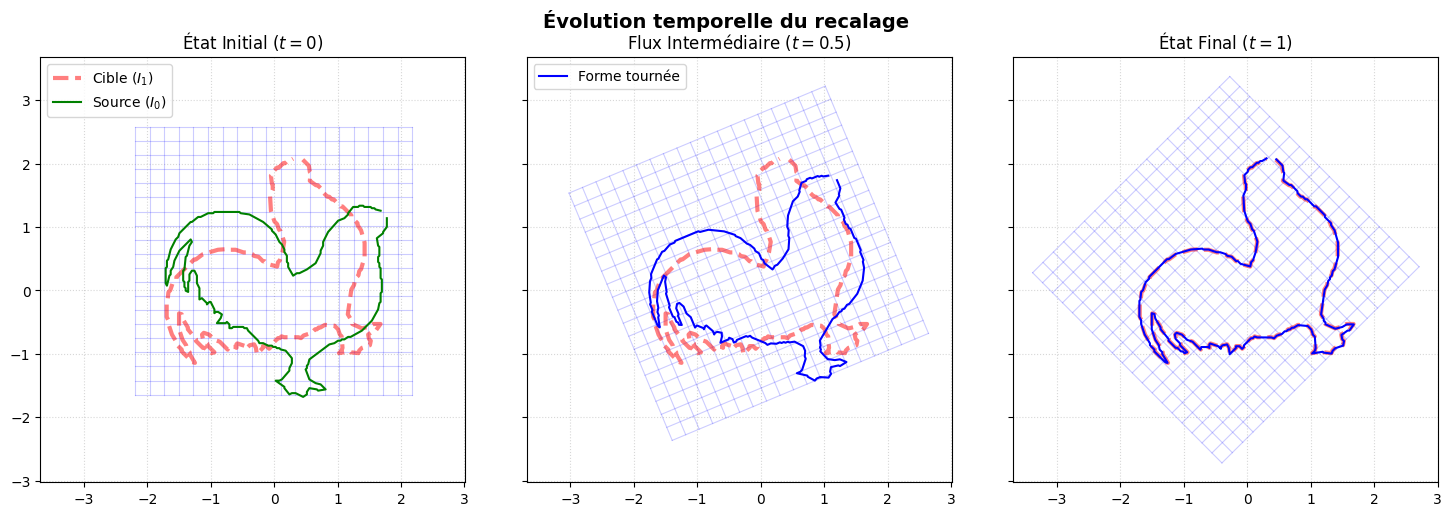
\includegraphics[width=1\textwidth]{../Images/EvolutionRecalageCoq0.png}
  \caption{Recalage sur les rotations $SO(2)$ d'un coq.}
\end{figure}
\end{exemple}


\section{Espace des formes, tangent et cotangent}
Dans la formulation géométrique du recalage, on considère un espace de champ de vecteurs $V\hookrightarrow C^{2}_{0}(\mathbb{R}^d,\mathbb{R}^d)$ et un espace de formes $Q$. Cet espace peut être, selon le problème étudié, un espace d'images, de courbes, de surfaces ou encore de nuage de points. Dans le cas des nuages de points, l'espace des formes est
\[
Q={(\mathbb{R}^d)}^N.
\]
Cet espace s'identifie naturellement à $\mathbb{R}^{dN}$. C'est donc un espace vectoriel normé de dimension finie où $N$ désigne le nombre de points et $d$ la dimension de l'espace ambiant. Comme tout espace vectoriel normé de dimension finie est complet, $\mathbb{R}^{dN}$ est un espace de Banach. Ainsi, $Q$ peut être vu comme une variété de Banach\footnote{Variété de Banach: Espace localement semblable à un espace de Banach}.\\
Pour décrire l'évolution des formes, on a besoin d'introduire les espaces tangents et cotangents.

\begin{definition}[Espace tangent de $Q$]\leavevmode\\
Puisque $Q$ est une variété (de Banach), on peut lui associer en tout point $q$ un espace tangent $T_{q}Q$, au sens de la définition générale~(\ref{def:espace-tangent}). On note
\[
TQ=\bigcup_{q\in Q} T_{q}Q=\{(q,v)\mid q\in Q, v\in T_{q}Q\}.
\]
\end{definition}

\begin{definition}[Espace cotangent de $Q$]\leavevmode\\
On définit son dual, l'espace cotangent $T_q^*Q$, qui est l'ensemble des formes linéaires sur $T_{q}Q$. On le définit par
\[
T^*Q=\bigcup_{q\in Q} T_q^*Q=\{(q,p)\mid q\in Q,\ p\in T_q^*Q\}.
\]
L'élément $p\in T_q^*Q$ est appelé un covecteur. Dans le cadre hamiltonien, on appelle ça un moment.
\end{definition}


\section{Problème variationnel LDDMM}
Le problème de recalage qui consiste a trouver la meilleure déformation peut s'écrire comme un problème variationnel où l'on doit déterminer le champ de vitesse $v_t$ qui minimise une énergie composée de deux termes:

\begin{itemize}
\item Un terme de régularité contrôlant le ``coût'' de la déformation (à gauche de l'addition),
\item Un terme d'attache aux données mesurant la similarité entre l'image transformée et la cible (à droite).
\end{itemize}
Le premier terme favorise des déformations douces, tandis que le second impose que la forme finale reste proche de la cible.\\
Le problème s'écrit:
\[
\begin{aligned}
\inf_{v\in L^2([0,1],V)}~&J(v)=\frac{1}{2}\int_{0}^{1}\|v_t\|_{V}^2\,dt+\|\varphi_1\cdot q_S-q_T\|_{L^2}\\
&\text{tel que }\left\{\begin{array}{ll}\dot{\varphi}_t=v_t\circ\varphi_t\\\varphi_0=Id\end{array}\right.
\end{aligned}
\]

\begin{theorem}\label{thm:min}
Notre problème ci-dessus admet un minimum.
\end{theorem}

\begin{proof}
Nous admettons le théorème et ne démontrons donc pas ce résultat ici. Piste de preuve: On utilise une méthode de calcul variationnel~\cite{MP25}, ``Direct method in the calculus of variations'' pour montrer que l'équation de minimisation admet un minimum, et en plus, le minimum est global.
\end{proof}

Réécrivons le problème en utilisant le \textit{Théorème~\ref{thm:min}}. On note $q_t=\varphi\cdot q_S$ la forme à l'instant $t$. L'action du champ de vecteurs $v_t$ sur la forme est notée $v_t\circ q_t$.\\
La dynamique du problème de recalage s'écrit alors
\[
\dot q_t = v_t\circ q_t.
\]
Le problème variationnel peut donc s'écrire sous la forme:
\[
\begin{aligned}
\min_{v\in L^2([0,1],V)}&\int_0^1 \|v_t\|_V^2\,dt + \mathcal{D}(q_1,q_T)\\
&\text{tel que }\left\{\begin{array}{ll}\dot q_t = v_t\circ q_t\\ q_0=q_S\end{array}\right.
\end{aligned}
\]
avec $\mathcal{D}$ une métrique adaptée aux données.\\
Ici, $q_S$ désigne encore la forme source et $q_T$ la forme cible.

\begin{remark}
Pour appliquer la méthode LDDMM, on n'a besoin que de l'action du groupe des difféomorphismes sur l'espace de formes. La formulation du problème de minimisation repose uniquement sur l'application du groupe à cet espace via $q_S \mapsto \varphi_1\cdot q_S$.
\end{remark}


\section{Formulation Hamiltonienne}
On peut interpréter le problème LDDMM comme un problème de contrôle optimal~\cite{TB16}. Dans ce cadre, le champ de vecteurs $v_t$ est le contrôle, tandis que la forme $q_t$ représente l'état du système. Son évolution est donnée par
\[
\dot q_t = v_t\circ q_t.
\]
Pour traiter ce problème contraint, on introduit un covecteur $p_t\in T_{q_t}^*Q$, appelé moment. Le Hamiltonien associé au problème de contrôle optimal noté
\[
H:T^*Q\times V\longrightarrow \mathbb{R}
\]
est défini par
\[
H(q,p,v)=(p\mid v\circ q)-\frac{1}{2}\|v\|_V^2.
\]
Le premier terme mesure l'interaction entre le moment $p$ et la vitesse de déformation $v\circ q$, tandis que le second représente le coût énergétique du champ de vecteurs $v$.

\subsection{Hamiltonien réduit}
Le principe du maximum de Pontryagin~\cite{Zib21} impose que le contrôle optimal maximise ce Hamiltonien par rapport à $v$. Pour obtenir cet Hamiltonien réduit en fonction de $q$ et $p$, on cherche d'abord le champ de vecteurs optimal $v^*$. Celui-ci est obtenu en annulant la dérivée de $H$ par rapport à la variable de contrôle $v$:
\[
\partial_v H(q,p,v)=0.
\]
On obtient ainsi un champ de vecteur optimal
\[
v^*=v^*(q,p).
\]
On remplace ensuite cette expression dans le hamiltonien initial pour définir le hamiltonien réduit
\[
H_r(q,p)=H(q,p,v^*(q,p)).
\]
Cette réduction permet de transformer le problème de contrôle optimal qui est en dimension infinie en un système d'équations différentielles sur $T^*Q$ qui est un problème en dimension finie.

\subsection{Équations géodésiques}
Les candidats à l'optimalité sont les géodésiques, c'est-à-dire des trajectoires satisfaisant les équations hamiltoniennes suivantes:
\[
\dot q_t = \partial_p H_r(q_t,p_t),
\]
\[
\dot p_t = -\partial_q H_r(q_t,p_t).
\]
La première équation décrit l'évolution de la forme. La seconde décrit l'évolution du moment associé. Dans le cadre LDDMM, la première équation redonne la dynamique
\[
\dot q_t = v_t\circ q_t.
\]

\begin{remark}
L'intérêt principal de la formulation hamiltonienne est qu'elle permet de remplacer l'optimisation sur le champ de vitesse $v_t$, qui appartient à un espace de dimension infinie, par l'étude d'un système différentiel portant sur les variables $(q_t,p_t)$.
\end{remark}

Ce chapitre a posé les fondements nécessaires à l'étude des cas particuliers, comme celui des rotations $SO(2)$ et $SO(3)$, qui seront abordés dans les chapitres suivants. En effet, dans ce rapport nous ne traitons pas le modèle LDDMM complet. Nous étudions une restriction de ce cadre dans le cas où les transformations considérées sont uniquement des rotations. Cette restriction permet d'obtenir un modèle plus simple que le modèle LDDMM complet qui repose sur l'action du groupe des difféomorphismes en dimension infinie.


% -= Lie =-
\chapter{\texorpdfstring{Le groupe $SO(n)$ et son algèbre de Lie $\mathfrak{so}(n)$}{Le groupe SO (n) et son algèbre de Lie so (n)}}

Dans ce chapitre, nous nous intéresserons aux particularités du groupe $SO(n)$ et de son algèbre de Lie $\mathfrak{so}(n)$ pour $n\geqslant 2$. Voici quelques définitions pour commencer.

\begin{definition} [Variété différentielle]\leavevmode\\
Une \textbf{variété différentielle} est un espace qui est localement assimilable\footnote{On pourrait aussi dire: localement homéomorphe à $\mathbb{R}^n$} à un espace euclidien~\cite{Hol24}.
\end{definition}

Considérons $G$ une variété différentielle.

\begin{definition} [Espace tangent]\label{def:espace-tangent}\leavevmode\\
On appelle \textbf{espace tangent} en $g$ à $G$, que l'on note $T_{g}G$, l'ensemble des vecteurs tangents en $g$.
\end{definition}

\begin{figure}[H]
  \centering
  \begin{tikzpicture}
    \begin{axis}[
      view={60}{30},
      axis lines=center,
      xlabel={$x$},
      ylabel={$y$},
      zlabel={$z$},
      xmin=-1.5, xmax=1.5,
      ymin=-1.5, ymax=1.5,
      zmin=-1.5, zmax=1.5,
      ticks=none,
      axis equal
      ]
      % Tracé de la sphère
      \addplot3[
          surf,
          colormap/viridis,
          samples=35,
          domain=0:360,
          y domain=0:180,
          z buffer=sort,
          opacity=0.7
      ] ({cos(x)*sin(y)}, {sin(x)*sin(y)}, {cos(y)});
      % Tracé du plan tangent
      \addplot3[
          surf,
          fill=cyan!40!white,
          faceted color=cyan!70!black,
          opacity=0.6,
          samples=2,
          domain=0.2:1.2,
          y domain=-0.5:0.5
      ] {1.4142 - x};
      % Point de tangence
      \addplot3[
          only marks,
          mark=*,
          mark size=1pt,
          color=blue
      ] coordinates {(0.7071, 0, 0.7071)};
    \end{axis}
  \end{tikzpicture}
  \caption{Figure du plan tangent à la sphère en un point.}
\end{figure}


% Groupe de Lie SO(n)
\section{\texorpdfstring{Le groupe de Lie $SO(n)$}{Le groupe de Lie SO (n)}}

Le \textbf{groupe spécial orthogonal} $SO(n)$ est un sous-groupe du \textbf{groupe orthogonal} $O(n)$. C'est le groupe des matrices de rotation à $n$ dimensions. On peut l'écrire:
\[
SO(n)=\{A\in \mathcal{M}_n(\mathbb{R})~|~\det{A}=1~;~A^{\top}A=I_n\}
\]

\begin{definition} [Groupe de Lie]\leavevmode\\
Un \textbf{groupe de Lie} est une variété différentielle qui est également un groupe, de telle sorte que l'opération de composition du groupe et l'opération d'inversion sont des applications lisses\footnote{Lisse: de classe $\mathcal{C}^{\infty}$}~\cite{Hol24}.
\end{definition}

\begin{theorem} [Théorème de submersion]\label{thm:submersion}\leavevmode\\
Soient $f\in \mathcal{C}^1(\mathbb{R}^n,\mathbb{R}^m)$ et $G := f^{-1}(e)$ où $e\in \mathbb{R}^m$.\\
Si $f$ est une submersion (i.e.~si $Df(x)$ est surjective en tout point $x$ de $G$), alors $G$ est une sous-variété de l'espace $\mathbb{R}^n$ de dimension $n-m$.
\end{theorem}

\begin{proof}
Admis
\end{proof}

\begin{proposition}\label{prop:SO-groupe-de-Lie}
$SO(n)$ est un groupe de Lie
\end{proposition}

\begin{proof}
Nous montrons d'abord que $SO(n)$ est un groupe (1), puis qu'il possède une structure de variété différentielle compatible avec les opérations de groupe (2). \medskip

(1) \textbf{$SO(n)$ est un groupe pour le produit matriciel.}\\
Soient $A,B\in SO(n)$, montrons que le produit est stable:
\[
{(AB)}^{\top}(AB)=B^{\top}A^{\top}AB=B^{\top}B=I_n\qquad\text{et}\qquad\det(AB)=\det(A)\det(B)=1.
\]
Ainsi $AB\in SO(n)$.\\
L'associativité est celle du produit matriciel.\\
L'élément neutre est la matrice identité $I_n$, qui appartient à $SO(n)$ puisque
\[
I_n^{\top}I_n=I_n\qquad\text{et}\qquad\det(I_n)=1.
\]
Enfin, si $A\in SO(n)$, alors
\[
A^{\top}A=I_n,
\]
d'où
\[
A^{-1}=A^{\top}.
\]
Comme
\[
\det(A^{-1})=\frac{1}{\det(A)}=1,
\]
on obtient $A^{-1}\in SO(n)$.\\
Ainsi \underline{$SO(n)$ est un groupe} et le produit matriciel est bien une loi de composition interne sur l'ensemble $SO(n)$.

\medskip
(2) \textbf{$SO(n)$ est une variété différentielle.}\\
Montrons que $SO(n)$ est muni d'une structure de variété différentielle, comme sous-variété de l'espace $\mathcal{M}_n(\mathbb{R})$.\\
Considérons l'application
\[
\begin{aligned}
f \colon \mathcal{M}_n(\mathbb{R}) &\longrightarrow \mathcal{S}_n(\mathbb{R})\\
X &\longmapsto X^{\top}X
\end{aligned}
\]
où $\mathcal{S}_n(\mathbb{R})$ désigne l'espace des matrices symétriques.\\
On remarque que
\[
O(n)=f^{-1}(I_n).
\]
Calculons la différentielle de $f$.\\
Soient $X\in O(n)$, et $H\in \mathcal{M}_n(\mathbb{R})$:
\[
\begin{aligned}
f(X+H)&={(X+H)}^{\top}(X+H)\\
&=X^{\top}X+X^{\top}H+H^{\top}X+H^{\top}H\\
&=f(X)+X^{\top}H+H^{\top}X+H^{\top}H
\end{aligned}
\]
Comme la norme subordonnée est sous-multiplicative
\[
\|H^{\top}H\|\leq\|H^{\top}\|\,\|H\|=\|H\|^2,
\]
on a
\[
\begin{aligned}
f(X+H)&=f(X)+X^{\top}H+H^{\top}X+O(\|H\|^2)\\
&=f(X)+Df(X)H+O(\|H\|^2)
\end{aligned}
\]
La différentielle de $f$ en $X$ est donc donnée par la partie linéaire en $H$,
\[
Df(X)H=X^{\top}H+H^{\top}X.
\]
Il reste à montrer que $f$ est une submersion en tout point de $O(n)$, donc que $Df(X)$ est surjective:\\
Soit $Y\in \mathcal{S}_n(\mathbb{R})$, déterminons $H$
\[
\begin{aligned}
Df(X)H=Y&\Leftrightarrow X^{\top}H+H^{\top}X=Y.
\end{aligned}
\]
Posons $H=\frac{1}{2}XY$ de telle sorte que pour $X\in O(n)$
\[
\begin{aligned}
Df(X)\frac{1}{2}XY=Y&\Leftrightarrow X^{\top}\frac{1}{2}XY+(\frac{1}{2}XY){}^{\top}X=Y\\
&\Leftrightarrow \frac{1}{2}X^{\top}XY+\frac{1}{2}Y^{\top}X^{\top}X=Y\\
\end{aligned}
\]
or $X^{\top}X=I_n$ et $Y^{\top}=Y$, donc
\[
Df(X)\frac{1}{2}XY=\frac{1}{2}I_{n}Y+\frac{1}{2}YI_n=Y.
\]
On a trouvé pour n'importe quel $Y$, qu'il y a un antécédent $H$. Ainsi, $Df$ est surjective et donc $O(n)$ est bien une sous-variété de l'espace $\mathcal{M}_n(\mathbb{R})$ (par le \textit{Théorème de submersion~\ref{thm:submersion}}).\\
Posons $U=\left\{A\in\mathcal{M}_n(\mathbb{R})\mid \det(A)>0\right\}$. Comme le déterminant est continu, $U$ est un ouvert de $\mathcal{M}_n(\mathbb{R})$. Or l'intersection d'une sous-variété avec un ouvert de l'espace ambiant est encore une sous-variété. Puisque
\[
SO(n)=O(n)\cap U,
\]
on en déduit que $SO(n)$ est une sous-variété de $\mathcal{M}_n(\mathbb{R})$.\\
Enfin, la structure de groupe de $SO(n)$ est compatible avec sa structure différentielle. En effet, l'application
\[
\begin{aligned}
\mu\colon SO(n)\times SO(n)&\longrightarrow SO(n),\\
(M,N)&\longmapsto MN^{-1}
\end{aligned}
\]
est lisse. Pour tout $N\in SO(n)$, on a $N^{-1}=N^\top$. Ainsi,
\[
\mu(M,N)=MN^\top.
\]
La transposition étant linéaire et la multiplication matricielle étant bilinéaire, ces deux opérations sont lisses. Par conséquent, $\mu$ est lisse. On a \underline{$SO(n)$ est un groupe de Lie}.
\end{proof}

\begin{remark}\label{rq:dim/tang}
Comme $SO(n)=O(n)\cap\{A\in\mathcal M_n(\mathbb R)\mid \det(A)>0\}$, le groupe $SO(n)$ est un ouvert de la variété $O(n)$. Il possède donc la même dimension que $O(n)$ et, en chaque point $X\in SO(n)$, le même espace tangent.\\
Par ailleurs, $O(n)=f^{-1}(I_n)$, où
\[
\begin{aligned}
f:\mathcal M_n(\mathbb R)&\longrightarrow\mathcal S_n(\mathbb R)\\
X&\longmapsto X^\top X
\end{aligned}
\]
Comme $I_n$ est une valeur régulière de $f$, le théorème des valeurs régulières donne
\[
\begin{aligned}
\dim SO(n)&=\dim O(n)\\
&=\dim\mathcal M_n(\mathbb R)-\dim\mathcal S_n(\mathbb R)\\
&=n^2-\frac{n(n+1)}{2}\\
&=\frac{n(n-1)}{2}
\end{aligned}
\]
\end{remark}


\subsection{Propriétés de l'action du groupe \texorpdfstring{$SO(n)$}{SO (n)} sur \texorpdfstring{$\mathbb{R}^n$}{Rn}}
Soient $G$ un groupe et $X$ un ensemble.

\begin{definition}[Action de groupe]\leavevmode\\
On dit que $G$ agit à gauche sur $X$ s'il existe une application $u\colon G\times X\longrightarrow X$ vérifiant
\begin{itemize}
  \item $u(e,x)=x$ pour tout $x\in X$ avec $e$ l'élément neutre de $G$,
  \item pour tout $g,g'\in G$ et $x\in X$
  \[
  u(g,u(g',x))=u(gg',x).
  \]
\end{itemize}
\end{definition}

\begin{remark}
On définit de même l'action à droite par la propriété $v(g,v(g',x))=v(g'g,x)$.
\end{remark}

\begin{proposition}
L'action naturelle du groupe $SO(n)$ sur $\mathbb{R}^n$ est donnée par la multiplication matricielle:
\[
\begin{aligned}
u\colon SO(n)\times \mathbb{R}^n&\longrightarrow \mathbb{R}^n\\
(R,x)&\longmapsto Rx
\end{aligned}
\]
\end{proposition}

\begin{proof}
Soient $R,R'\in SO(n)$ et $x\in \mathbb{R}^n$,
\[
u(I_n,x)=I_{n}x=x.
\]
Et
\[
u(R,u(R',x))=u(R,R'x)=RR'x=u(RR',x).
\]
La multiplication matricielle \underline{$u$ est une action de groupe}.
\end{proof}

\begin{proposition}
L'action du groupe $SO(n)$ dans $\mathbb{R}^n$ est fidèle mais pas libre et pas transitive.
\end{proposition}

\begin{proof}
L'action de $SO(n)$ dans $\mathbb{R}^n$ est \textbf{fidèle}:\\
Si l'action est fidèle, alors si $R\in SO(n)$ tel que $u(R,x)=x, \forall x\in \mathbb{R}^n$ alors $R=I_n$.\\
Supposons que $R\in SO(n)$ vérifie $Rx=x$ pour tout $x\in \mathbb{R}^n$. Alors, pour tout vecteur de la base canonique de $\mathbb{R}^n$: $(e_1,\dots,e_n)$, on a
\[
Re_i = e_i \quad \forall~1\leq i\leq n.
\]
Ainsi, les colonnes de $R$ sont celles de l'identité, donc $R=I_n$.~\underline{L'action est fidèle}.\\

L'action de $SO(n)$ dans $\mathbb{R}^n$ n'est \textbf{pas libre}:\\
Si l'action est libre, alors pour tout $x\in \mathbb{R}^n$, si $x\neq 0$ et $R\neq I_n$ alors $Rx\neq x$.\\
Pour $n=2$, cette action est libre: une rotation plane qui fixe un vecteur non nul est nécessairement l'identité.\\
En revanche, pour $n\geq3$. Prenons $R=\begin{pmatrix} 1 & 0 \\ 0 & S \end{pmatrix}$ une matrice par bloc de $SO(n)$ où $S\in SO(n-1)$ différente de l'identité et $x=(1,0,\dots ,0)$.\\
Alors $u(R,x)=Rx=x$ car $x$ est dans la direction de la première colonne de $R$.\\
Donc \underline{l'action de $SO(n)$ dans $\mathbb{R}^n$ n'est pas libre}.\\

L'action de $SO(n)$ dans $\mathbb{R}^n$ n'est \textbf{pas transitive}:\\
Si l'action est transitive, alors $\forall x,y\in \mathbb{R}^n, \exists R\in SO(n)$ tel que $u(R,x)=y$.\\
Prenons $x=0$ et $y=(1,0,\dots ,0)$.\\
Alors $\forall R\in SO(n)$, $u(R,x)=Rx=R\cdot 0=0\neq y$.\\
Donc \underline{l'action de $SO(n)$ dans $\mathbb{R}^n$ n'est pas transitive}.
\end{proof}

\begin{proposition}
L'action de $SO(n)$ sur $\mathbb{R}^n$ est isométrique. C'est-à-dire:
\[
\forall x,y\in \mathbb{R}^n, \forall R\in SO(n), \left\langle Rx,Ry\right\rangle=\left\langle x,y\right\rangle.
\]
\end{proposition}

\begin{proof}
Soient $x,y\in \mathbb{R}^n$ et $R\in SO(n)$\\
\[
\left\langle Rx,Ry\right\rangle=\left\langle x,R^{\top}Ry\right\rangle.
\]
Or $R^{\top}R=I_n$ car $R\in SO(n)$, donc
\[
\begin{aligned}
\left\langle Rx,Ry\right\rangle&=\left\langle x,I_{n}y\right\rangle\\
&=\left\langle x,y\right\rangle.
\end{aligned}
\]
\underline{L'action de $SO(n)$ sur $\mathbb{R}^n$ est isométrique}, elle préserve bien la distance.
\end{proof}

\begin{definition}[Orbite d'une action]\leavevmode\\
On appelle \textbf{orbite de $x$} la partie de l'ensemble $X$ définie par
\[
Orb(x)=\{u(g,x)~|~g\in G\}.
\]
\end{definition}

\begin{proposition}
Les orbites de l'action naturelle de $SO(n)$ sur $\mathbb{R}^n$ sont les sphères centrées en l'origine. Plus précisément, pour tout $x\in\mathbb{R}^n$,
\[
\operatorname{Orb}(x)=\{Rx \mid R\in SO(n)\}=\{y\in\mathbb{R}^n \mid \|y\|=\|x\|\}.
\]
En particulier, si $x=0$, alors
\[
\operatorname{Orb}(0)=\{0\}.
\]
\end{proposition}

\begin{proof}
Soit $x\in\mathbb{R}^n$. Montrons par double inclusion:

\underline{$\operatorname{Orb}(x)\subset\{z\in\mathbb{R}^n \mid \|z\|=\|x\|\}$}: Soit $y\in \operatorname{Orb}(x)$. Alors il existe $R\in SO(n)$ tel que
\[
y=Rx.
\]
Comme l'action de $SO(n)$ sur $\mathbb{R}^n$ est isométrique, on a
\[
\|y\|=\|Rx\|=\|x\|.
\]
Donc
\[
y\in \{z\in\mathbb{R}^n \mid \|z\|=\|x\|\}.
\]
Ainsi,
\[
\operatorname{Orb}(x)\subset\{z\in\mathbb{R}^n \mid \|z\|=\|x\|\}.
\]

\underline{$\operatorname{Orb}(x)\supset\{z\in\mathbb{R}^n \mid \|z\|=\|x\|\}$}: Soit maintenant $y\in\mathbb{R}^n$ tel que
\[
\|y\|=\|x\|.
\]
Si $x=0$, alors $\|y\|=0$, donc $y=0$. On a donc bien
\[
\operatorname{Orb}(0)=\{0\}.
\]
Supposons maintenant que $x\neq 0$. Alors $y\neq 0$ également. Les vecteurs
\[
\frac{x}{\|x\|}\qquad\text{et}\qquad\frac{y}{\|y\|}
\]
sont deux vecteurs unitaires de $\mathbb{R}^n$. On peut compléter chacun d'eux en une base orthonormée directe de $\mathbb{R}^n$:
\[
\mathcal{B}_x=\left(\frac{x}{\|x\|},e_2,\dots,e_n\right),\qquad\mathcal{B}_y=\left(\frac{y}{\|y\|},f_2,\dots,f_n\right).
\]
Il existe alors une matrice $R\in SO(n)$ envoyant la base $\mathcal{B}_x$ sur la base $\mathcal{B}_y$. En particulier,
\[
R\left(\frac{x}{\|x\|}\right)=\frac{y}{\|y\|}.
\]
Comme $\|x\|=\|y\|$, on obtient
\[
Rx=y.
\]
Donc $y\in \operatorname{Orb}(x)$.\\
Ainsi,
\[
\{z\in\mathbb{R}^n \mid \|z\|=\|x\|\}\subset\operatorname{Orb}(x).
\]

Finalement, les deux inclusions donnent \underline{$\operatorname{Orb}(x)=\{y\in\mathbb{R}^n \mid \|y\|=\|x\|\}$}.
\end{proof}


\subsection{Propriétés topologiques de \texorpdfstring{$SO(n)$}{SO (n)}}

\begin{theorem}[Compacité en dimension finie]\label{thm:compact-dim-finie}\leavevmode\\
Soient $(X,\|~\|)$ un espace vectoriel normé de dimension finie et $E\subset X$ une partie de $X$. Alors $E$ est compacte si et seulement si $E$ est fermée et bornée. 
\end{theorem}

\begin{proof}
$\Rightarrow$ Une partie compacte est aussi fermée et bornée. Cette implication est donc vraie dans n'importe quel espace.

$\Leftarrow$ C'est une conséquence du Théorème de Bolzano-Weierstrass.
\end{proof}

\begin{proposition}\label{prop:SO-compact}
$SO(n)$ est un groupe compact.
\end{proposition}

\begin{proof}
On a $SO(n)\subset \mathcal{M}_n(\mathbb{R})$ qui est en dimension finie.\\
Montrons que $SO(n)$ est fermé (1) et borné (2):

(1) $SO(n)$ \textbf{fermé}.\\
Soient $f$ et $g$ deux applications continues.
\[
\begin{aligned}
f \colon \mathcal{M}_n(\mathbb{R}) &\longrightarrow \mathbb{R}~&g \colon \mathcal{M}_n(\mathbb{R}) &\longrightarrow \mathcal{M}_n(\mathbb{R})\\
X &\longmapsto \det(X)&X &\longmapsto X^{\top}X
\end{aligned}
\]
On pose $\{1\}\subset\mathbb{R}$ et $\{I_n\}\subset\mathcal{M}_n(\mathbb{R})$, deux fermés (car ce sont des singletons).\\
Alors $SO(n)=f^{-1}(\{1\})\cap g^{-1}(\{I_n\})$, comme l'intersection de deux fermés (images réciproques de fermés par des applications continues).
Ainsi \underline{$SO(n)$ est fermé}.\\

(2) $SO(n)$ \textbf{borné}.\\
Soit $A\in SO(n)$, alors $\|A\|_F^2=\operatorname{Tr}(A^{\top}A)=\operatorname{Tr}(I_n)=n$.\\
On a donc: $\forall A\in SO(n), \exists M=\sqrt{n}$ tel que $\|A\|\leq M$ (toutes les normes sont équivalentes en dimension finie).\\
On retrouve que \underline{$SO(n)$ est borné} car $SO(n)\subset B(0,M)$.\\

Finalement, $SO(n)$ fermé et borné donc (par le \textit{Théorème de compacité en dimension finie~\ref{thm:compact-dim-finie}}) \underline{$SO(n)$ est compact}.
\end{proof}

\begin{proposition}\label{prop:SO-connexe-arcs}
$SO(n)$ est un groupe connexe par arcs.
\end{proposition}

\begin{proof}
On procède par récurrence sur $n \ge 1$ en utilisant l'action naturelle de $SO(n)$ sur la sphère $S^{n-1}\subset \mathbb{R}^n$.
\[
\begin{aligned}
u\colon SO(n)\times S^{n-1} &\longrightarrow S^{n-1}\\
(A,x) &\longmapsto Ax
\end{aligned}
\]
Pour $n = 1$, le groupe $SO(1) = \{1\}$ est un singleton, il est donc trivialement connexe par arcs.\\\\
Vérifions que le fixateur du vecteur $e_n ={(0,\dots,0,1)}^{\top}$ s'identifie à $SO(n-1)$.\\
Une matrice $A \in SO(n)$ vérifie $Ae_n = e_n$ si et seulement si sa dernière colonne est $e_n$. Étant orthogonale, ses lignes et colonnes forment des familles orthonormées, ce qui impose à $A$ d'avoir une structure de bloc de la forme:
\[
A = \begin{pmatrix} B & 0 \\ 0 & 1 \end{pmatrix}
\]
où $B \in \mathcal{M}_{n-1}(\mathbb{R})$. Les conditions $A^{\top}A=I_n$ et $\det(A)=1$ sont aussi vérifiées sur le bloc $B$.\\
Donc, $B \in SO(n-1)$. L'application $B \mapsto \begin{pmatrix} B & 0 \\ 0 & 1 \end{pmatrix}$ définit un isomorphisme qui permet d'identifier le fixateur de $e_n$ à $SO(n-1)$.\\\\
Montrons que l'application $SO(n)/SO(n-1)\longrightarrow S^{n-1}$ ainsi obtenue est un homéomorphisme.\\
L'action de $SO(n)$ sur $S^{n-1}$ est transitive pour tout $n \ge 2$ (tout vecteur unitaire peut être complété en une base orthonormée). L'application associée à $e_n$ est donc surjective:
\[
\begin{aligned}
\varphi \colon SO(n) &\longrightarrow S^{n-1}\\
\quad A &\longmapsto Ae_n
\end{aligned}
\]
Par passage au quotient, $\varphi$ induit une bijection continue:
\[
\varphi' \colon SO(n)/SO(n-1) \longrightarrow S^{n-1}
\]
Le groupe $SO(n)$ étant compact~(\ref{prop:SO-compact}), toute bijection continue d'un espace compact vers un espace séparé est un homéomorphisme.\\
On en déduit que $SO(n)/SO(n-1) \simeq S^{n-1}$.\\\\
Montrons que si $H$ est un sous-groupe fermé connexe de $G$, l'application quotient induit une bijection $\pi_0(G)\simeq \pi_0(G/H)$.\\
En effet, soit $f \colon G \to \{0, 1\}$ une application continue. Pour tout $g \in G$, la restriction de $f$ à la classe $gH$ est continue. Comme $H$ est connexe, la fibre\footnote{En topologie, la fibre d'un point par une application désigne simplement sa préimage} $gH$ est connexe, donc $f$ est constante. Donc, $f$ passe au quotient en une application continue $\bar{f}$. Si $G/H$ est connexe, $\bar{f}$ est constante, impliquant que $f$ est constante sur $G$.\\
$G$ est donc connexe.\\\\
On en déduit la connexité de $SO(n)$ par récurrence.\\
Supposons que $SO(n-1)$ est connexe. On applique l'égalité précédente à $G=SO(n)$ et $H=SO(n-1)$.\\
Par hypothèse, $H$ est connexe. De plus, pour $n \ge 2$, l'espace quotient $SO(n)/SO(n-1) \simeq S^{n-1}$ est connexe.\\
\underline{$SO(n)$ est donc connexe}.\\\\
Et \underline{$SO(n)$ est connexe par arcs} car c'est une variété différentielle~(\ref{prop:SO-groupe-de-Lie}) localement connexe par arcs et compacte~(\ref{prop:SO-compact}).
\end{proof}


% Algèbre de Lie so(n)
\section{L'algèbre de Lie \texorpdfstring{$\mathfrak{so}(n)$}{so (n)}}

L'outil principal qui nous permettra d'étudier les groupes de Lie est leur algèbre de Lie. Définissons cette structure pour les rotations et intéressons-nous aux propriétés différentielles des groupes de Lie. Prenons $G$ un groupe de Lie et $e\in G$ son élément neutre.

\begin{definition} [Algèbre de Lie]\leavevmode\\
Une \textbf{algèbre de Lie}, notée $\mathfrak{g} = T_{e}G$, est un espace vectoriel muni d'un produit appelé crochet de Lie, qui est une application bilinéaire antisymétrique~\cite{Hol24}
\[
[\cdot,\cdot] : \mathfrak{g} \times \mathfrak{g} \to \mathfrak{g}
\]
et qui satisfait l'identité de Jacobi:
\[
[\xi,[\eta, \zeta]] + [\eta,[\zeta, \xi]] + [\zeta,[\xi, \eta]] = 0, \quad \text{pour } (\xi,\eta,\zeta) \in \mathfrak{g}^3.
\]
\end{definition}

\begin{proposition}\label{prop:so(n)=o(n)}
Les algèbres de Lie des groupes $SO(n)$ et $O(n)$ coïncident:
\[
\mathfrak{so}(n)=\mathfrak{o}(n)
\]
\end{proposition}

\begin{proof}
Montrons par double inclusion:

$\mathfrak{so}(n)\subset \mathfrak{o}(n)$: Comme $SO(n)\subset O(n)$, tout vecteur tangent à $SO(n)$ en l'identité est aussi tangent à $O(n)$.
\[
T_{I_n}SO(n)\subset T_{I_n}O(n),~\text{donc}~\mathfrak{so}(n)\subset \mathfrak{o}(n).
\]

$\mathfrak{so}(n)\supset \mathfrak{o}(n)$: On utilise le fait que $SO(n)$ est la composante connexe de l'identité dans $O(n)$~(\ref{prop:SO-connexe-arcs}).\\
Au voisinage de $I_n$, la condition $\det X=1$ dans $O(n)$ est automatiquement satisfaite sur la composante où $\det X>0$. Comme le déterminant est continu et vaut $1$ en $I_n$, il existe un voisinage de $I_n$ dans lequel tout élément de $O(n)$ a un déterminant positif, donc égal à $1$ puisqu'un élément de $O(n)$ a un déterminant $\pm 1$. Ainsi, $O(n)$ et $SO(n)$ coïncident localement au voisinage de $I_n$. Ils ont donc le même espace tangent en $I_n$.

Finalement, on a \underline{$\mathfrak{so}(n)=\mathfrak{o}(n)$}.
\end{proof}

\begin{proposition}
$T_{I_n}SO(n)=\{H\in \mathcal{M}_n(\mathbb{R})~|~H^{\top}=-H\}$ est l'algèbre de Lie de $SO(n)$, plus précisément: $\mathfrak{so}(n)=T_{I_n}SO(n)$.
\end{proposition}

\begin{proof}
$SO(n)$ est un groupe de Lie~(\ref{prop:SO-groupe-de-Lie}). L'algèbre de Lie d'un groupe de Lie est définie comme son espace tangent en l'identité (ici $Id$), que l'on trouve en différenciant $f$\footnote{En effet, on peut ignorer la condition sur le déterminant car on a déjà montré que les algèbres de Lie de $SO(n)$ et $O(n)$ coïncident~(\ref{prop:so(n)=o(n)})} en l'identité avec
\[
\begin{aligned}
f \colon \mathcal{M}_n(\mathbb{R}) &\longrightarrow \mathcal{S}_n(\mathbb{R})\\
X &\longmapsto X^{\top}X
\end{aligned}
\]
Par la preuve de la \textit{proposition~(\ref{prop:SO-groupe-de-Lie})}, on a
\[
Df(X)H=X^{\top}H+H^{\top}X.
\]
On l'évalue en l'identité
\[
Df(I_n)H=I_n^{\top}H+H^{\top}I_n=H+H^{\top}.
\]
Et comme
\[
O(n)=f^{-1}(I_n)
\]
et que $I_n$ est une valeur régulière de $f$, le théorème des valeurs régulières donne, pour tout $X\in O(n)$,
\[
T_{X}O(n)=\ker(Df(X)).
\]
Par~(\ref{rq:dim/tang}), on a
\[
T_{I_n}SO(n)=T_{I_n}O(n)=\ker Df(I_n).
\]
Enfin,
\[
T_{I_n}SO(n)=\ker(Df(I_n))=\{H\in\mathcal{M}_n(\mathbb{R})~|~H^{\top}=-H\}
\]
Par définition, l'algèbre de Lie de $SO(n)$ est l'espace tangent en l'identité.\\
Ainsi, l'algèbre de Lie du groupe des rotations de dimension $n$ est l'ensemble des matrices antisymétriques.
\[
\mathfrak{so}(n)=\{H\in\mathcal{M}_n(\mathbb{R})~|~H^{\top}=-H\}
\]
\end{proof}

\begin{definition} [Crochet de Lie dans $\mathfrak{so}(n)$]\leavevmode\\
Le commutateur de $\mathfrak{so}(n)$ est, pour $A,B\in\mathfrak{so}(n)$:
\[
\begin{aligned}
(\relax[\cdot,\cdot]) : \mathfrak{g} \times \mathfrak{g} &\to \mathfrak{g}\\
(A,B) &\mapsto  AB-BA
\end{aligned}
\]
\end{definition}

\begin{proposition}
Si $A,B\in \mathfrak{so}(n)$, Alors $[A,B]\in\mathfrak{so}(n)$
\end{proposition}

\begin{proof}
Soient $A,B\in \mathfrak{so}(n)$, calculons la transposée de $[A,B]$
\[
\begin{aligned}
{[A,B]}^{\top}&={(AB-BA)}^{\top}\\
&={(AB)}^{\top}-{(BA)}^{\top}\\
&=B^{\top}A^{\top}-A^{\top}B^{\top}.
\end{aligned}
\]
On utilise l'antisymétrie de $A$ et $B$
\[
\begin{aligned}
{[A,B]}^{\top}&=(-B)(-A)-(-A)(-B)\\
&=-(AB-BA)=-[A,B]
\end{aligned}
\]
On a bien $[A,B]$ antisymétrique, donc \underline{$[A,B]\in\mathfrak{so}(n)$}.
\end{proof}

\begin{definition}[Translation à droite]\label{def:translation}\leavevmode\\
Soit $g\in G$. On note \textbf{translation à droite} l'application:
\[
\begin{aligned}
R_g\colon G &\longrightarrow G\\
h&\longmapsto hg
\end{aligned}
\]
\end{definition}

\begin{proposition}\label{prop:translation-lisse}
La translation à droite sur le groupe $SO(n)$ est une application lisse.
\end{proposition}

\begin{proof}
Soit $R_M$ une translation à droite sur $SO(n)$. On peut définir cette translation comme:
\[
\begin{aligned}
R_M\colon SO(n) &\longrightarrow SO(n)\\
X&\longmapsto u\times v=XM
\end{aligned}
\]
Par produit lisse (car c'est une application polynomiale en les coefficients), on a que \underline{$R_M$ est une application lisse} sur $SO(n)$.
\end{proof}

\begin{proposition}\label{prop:Tangent-isomorphe}
L'espace $T_{M}SO(n)$ est isomorphe à $T_{I_n}SO(n)$ pour tout $M\in SO(n)$
\end{proposition}

\begin{proof}
Soit $M \in SO(n)$. On considère la translation à droite~(\ref{def:translation}) sur $SO(n)$ définie par
\[
\begin{aligned}
R_M : SO(n) &\longrightarrow SO(n)\\
X &\longmapsto XM
\end{aligned}
\]
Cette application est lisse~(\ref{prop:translation-lisse}), et son inverse $R_{M^{-1}}$ est lisse. Ainsi, $R_M$ est un difféomorphisme de $SO(n)$.\\
En particulier, sa différentielle en tout point est un isomorphisme linéaire. En évaluant en l'identité, on obtient
\[
{(dR_M)}_{I_n} : T_{I_n}SO(n) \longrightarrow T_M SO(n),
\]
qui est un isomorphisme.
Son inverse est donné par
\[
{(dR_{M^{-1}})}_{M} : T_M SO(n) \longrightarrow T_{I_n}SO(n),
\]
et par théorème de dérivation des fonctions composées, on a
\[
\begin{aligned}
{(dR_{M^{-1}})}_M\circ{(dR_M)}_{I_n}
&=d{(R_{M^{-1}}\circ R_M)}_{I_n}\\
&=d{(\operatorname{Id}_{SO(n)})}_{I_n}\\
&=\operatorname{Id}_{T_{I_n}SO(n)}
\end{aligned}
\]
On en déduit que $T_M SO(n)$ et $T_{I_n}SO(n)$ sont isomorphes.
\end{proof}

\begin{remark}
La translation à droite permet de ``passer''\footnote{Passer: transporter de manière isomorphe les structures} d'un espace tangent à un autre, reliant l'espace tangent en un point quelconque et l'espace tangent à l'identité~(\ref{prop:Tangent-isomorphe}).
\end{remark}

\begin{exemple}
La figure ci-dessous \texttt{Figure~(\ref{fig:espaces-tangents})} illustre ce principe sur la surface $z=x^2-y^2$ (qui joue ici le rôle d'une variété différentielle). Le long de la courbe $y=1$, on a représenté les plans tangents ${T}_{g_0}G$ et ${T}_{g_t}G$ en $g_0=(-2,1,3)$ et $g_t=(0,1,-1)$, ainsi que les vecteurs tangents correspondants. Le passage de l'un à l'autre peut être réalisé par une translation à droite convenable.
\end{exemple}

\begin{figure}[H]
  \centering
  \begin{tikzpicture}
  \begin{axis}[
      view={120}{30},
      xlabel=$x$, ylabel=$y$, zlabel=$z$,
      colormap/viridis,
      grid=major,
      clip=false,
  ]
  % Surface principale
  \addplot3[
      surf,
      shader=interp,
      samples=40,
      domain=-2:2,
      domain y=-2:2,
      opacity=0.8
  ]
  {x^2 - y^2};
  % Plan tangent en g_0
  \addplot3[
      surf,
      faceted color=blue,
      fill opacity=0.3,
      draw opacity=0.2,
      samples=15,
      domain=-2.5:-1.5,
      domain y=0.5:1.5
  ]
  {-4*x -2*y -3};
  % Plan tangent en g_t
  \addplot3[
      surf,
      faceted color=blue,
      fill opacity=0.3,
      draw opacity=0.2,
      samples=15,
      domain=-0.8:0.8,
      domain y=0.5:1.5
  ]
  {-2*y +1};
  % Courbe sur la surface (y=1)
  \addplot3[
      color=red,
      thick,
      domain=-2:2,
      samples=50,
      samples y=0,
  ]
  ({x}, 1, {x^2 - 1});
  % Points g_0, g_t, g_1
  \addplot3[only marks, mark=*, mark size=2.5, color=red] coordinates {
      (-2,1,3)  % g_0
      (0,1,-1)  % g_t
      (2,1,3)   % g_1
  };
  % Étiquettes des points
  \node[anchor=south west] at (axis cs:-2,1,3) {$\mathbf{g}_0$};
  \node[anchor=north]      at (axis cs:0,1,-1) {$\mathbf{g}_t$};
  \node[anchor=south east] at (axis cs:2,1,3) {$\mathbf{g}_1$};
  % Vecteur tangent en g_0
  \draw[->, thick, blue] (axis cs:-2,1,3) -- (axis cs:-1.75,1,2);
  \node[anchor=south east, blue] at (axis cs:-1.75,1,2) {$\mathbf{T}_{g_0}G$};
  % Vecteur tangent en g_t
  \draw[->, thick, blue] (axis cs:0,1,-1) -- (axis cs:0.5,1,-1);
  \node[anchor=south, blue] at (axis cs:0.5,1,0) {$\mathbf{T}_{g_t}G$};
  \end{axis}
  \end{tikzpicture}
  \caption{Figure des plans tangents à une surface en $g_0$ et $g_t$.}\label{fig:espaces-tangents}
\end{figure}


% Exponentielle
\section{L'application exponentielle}

\begin{definition} [Exponentielle de matrice]\label{def:exp-matrix}\leavevmode\\
Soit $A\in \mathcal{M}_n(\mathbb{K})$ avec $\mathbb{K}=\mathbb{R}$ ou $\mathbb{C}$.  On appelle exponentielle de la matrice $A$, notée $e^A$, la somme de la série:
\[
e^{A}=\sum_{k=0}^{\infty}\frac{A^k}{k!}~,\qquad \exp(0)=I_n.
\]
\end{definition}

\begin{proposition}\label{prop:ensemble-exp}
Si $A\in\mathfrak{so}(n)$, Alors $e^A\in SO(n)$.
\end{proposition}

\begin{proof}
Montrons que $\det(e^A)=1$ et ${(e^A)}^{\top}e^A=I_n$, et donc que $e^A\in SO(n)$.\\
Soit $A\in \mathfrak{so}(n)$, $A$ est une matrice antisymétrique.\\
On sait que pour tout $M\in \mathcal{M}_n(\mathbb{R})$
\[
\det(e^M)=e^{\operatorname{Tr}(M)}.
\]
Par antisymétrie de $A$, $\operatorname{Tr}(A)=0$.\\
Et donc
\[
\det(e^A)=e^{\operatorname{Tr}(A)}=e^0=1.
\]
Maintenant, montrons que ${(e^A)}^{\top}e^A=I_n$.\\
Pour la même matrice $A$,
\[
\begin{aligned}
{(e^A)}^{\top}&={\left( \sum_{k=0}^{\infty}\frac{A^k}{k!}\right)}^{\top}=\sum_{k=0}^{\infty}\frac{{(A^k)}^{\top}}{k!}\\
&=\sum_{k=0}^{\infty}\frac{{({A}^{\top})}^k}{k!}=e^{(A^{\top})}.
\end{aligned}
\]
Or $A^{\top}=-A$,
\[
{(e^A)}^{\top}(e^A)=(e^{-A})(e^A)=e^0=I_n.
\]
Ainsi, $e^A$ vérifie $\det(e^A)=1$ et ${(e^A)}^{\top}e^A=I_n$.\\
On a bien \underline{$e^A\in SO(n)$}.
\end{proof}

\begin{exemple}
Exemple d'exponentielle d'une matrice $2\times 2$ antisymétrique:\\
Soient $\theta\in\mathbb{R}$ et $A=\begin{pmatrix}0 & -\theta\\\theta & 0\end{pmatrix}\in\mathfrak{so}(2)$. Calculons $e^{A}$:\\
On observe que
\[
A^{2}=\begin{pmatrix} -\theta^{2} & 0 \\ 0 & -\theta^{2} \end{pmatrix} = -\theta^{2} I_{2},
\]
et par récurrence,
\[
A^{2k}={(-1)}^{k}\theta^{2k} I_{2},\qquad A^{2k+1}={(-1)}^{k}\theta^{2k+1} \begin{pmatrix} 0 & -1 \\ 1 & 0 \end{pmatrix}.
\]
Alors
\[
\begin{aligned}
e^{A} &= \sum_{k=0}^{\infty} \frac{A^{k}}{k!}= \sum_{k=0}^{\infty} \frac{A^{2k}}{(2k)!} + \sum_{k=0}^{\infty} \frac{A^{2k+1}}{(2k+1)!}\\
&= \left( \sum_{k=0}^{\infty} \frac{{(-1)}^{k}\theta^{2k}}{(2k)!} \right) I_{2}\;+\; \left( \sum_{k=0}^{\infty} \frac{{(-1)}^{k}\theta^{2k+1}}{(2k+1)!} \right)\begin{pmatrix} 0 & -1 \\ 1 & 0 \end{pmatrix}.
\end{aligned}
\]
On reconnaît les séries du cosinus et du sinus:
\[
\cos\theta=\sum_{k=0}^{\infty} \frac{{(-1)}^{k}\theta^{2k}}{(2k)!},\qquad\sin\theta=\sum_{k=0}^{\infty} \frac{{(-1)}^{k}\theta^{2k+1}}{(2k+1)!}.
\]
Ainsi,
\[
e^{A}=\cos\theta\;I_{2}+\sin\theta \begin{pmatrix} 0 & -1 \\ 1 & 0 \end{pmatrix}=\begin{pmatrix} \cos\theta & -\sin\theta \\ \sin\theta & \cos\theta \end{pmatrix},
\]
qui est bien une matrice de rotation, donc $e^A\in SO(2)$.
\end{exemple}

\begin{proposition}
L'application exponentielle $\exp \colon \mathfrak{so}(n)\longrightarrow SO(n)$ est surjective.
\end{proposition}

\begin{proof}
Soit $R\in SO(n)$. Par le théorème spectral, il existe une base orthonormée dans laquelle la matrice de $R$ est diagonale par blocs, les blocs diagonaux étant soit des blocs de rotation:
\[
R(\theta_k)=\begin{pmatrix}\cos\theta_k & -\sin\theta_k\\\sin\theta_k & \cos\theta_k\end{pmatrix},
\]
soit des blocs $(1)$ et $(-1)$.\\
Comme $\det R=1$, les valeurs propres $(-1)$ apparaissent en nombre pair; on les regroupe donc deux à deux pour former des blocs
\[
-I_2=R(\pi).
\]
On obtient ainsi une décomposition
\[
R=P\,\mathrm{diag}\bigl(R(\theta_1),\ldots,R(\theta_r),1,\ldots,1\bigr)P^{-1},
\]
où $P$ est orthogonale.\\
Pour chaque bloc de rotation d'angle $\theta_k$, on construit explicitement
\[
A_k=\begin{pmatrix}0 & -\theta_k\\\theta_k & 0\end{pmatrix}\in \mathfrak{so}(2),
\]
de sorte que
\[
e^{A_k}=R(\theta_k).
\]
On pose alors
\[
A=P\,\mathrm{diag}(A_1,\ldots,A_r,0,\ldots,0)\,P^{-1}.
\]
Comme $\mathfrak{so}(n)$ est stable par conjugaison orthogonale, on a $A\in\mathfrak{so}(n)$.\\
Finalement,
\[
e^A=P\,\mathrm{diag}\bigl(e^{A_1},\ldots,e^{A_r},1,\ldots,1\bigr)P^{-1}=R.
\]
Ainsi, on retrouve que $e^A=R$, et donc que pour tout $R\in SO(n)$, il existe $A\in\mathfrak{so}(n)$ tel que $e^A=R$.~\underline{L'exponentielle est surjective} de l'algèbre de Lie de $SO(n)$ dans son groupe de Lie.
\end{proof}


% -= Equa diff =-
\chapter{Étude de l'équation différentielle linéaire \texorpdfstring{$\dot{x}(t)=Ax(t)$}{x.\ (t)=Ax (t)}}

Dans ce chapitre, nous verrons comment cette équation différentielle linéaire apparaît naturellement sur le groupe spécial orthogonal $SO(n)$, l'importance de ce résultat, ainsi que sa résolution. Commençons avec le groupe de Lie $SO(n)$.


\section{Obtenir l'équation différentielle \texorpdfstring{$\dot{x}(t)=Ax(t)$}{x.\ (t)=Ax (t)}}

Cherchons à exprimer la différentielle de la translation à droite afin de lier le groupe $SO(n)$ à son algèbre de Lie. Remarquons une égalité que l'on utilisera juste après.
\begin{remark}\label{rq:id}
On sait que $\forall X\in SO(n)\colon X^{\top}X=I_n$, et donc $X^{-1}=X^{\top}$.
\end{remark}
\subsubsection{Trouvons l'équation.}
Prenons la translation à droite sur $SO(n)$ avec $M\in SO(n)$:
\[
\begin{aligned}
R_M\colon SO(n) &\longrightarrow SO(n)\\
X&\longmapsto XM
\end{aligned}
\]
Différencions cette application, soient $X\in SO(n)$ et $H\in \mathcal{M}_n(\mathbb{R})$
\[
\begin{aligned}
R_M(X+H)&=(X+H)M\\
&=XM+HM\\
&=R_M(X)+DR_M(X)H+o(\|H\|)
\end{aligned}
\]
La différentielle de $R_M$ en $X$ est donc donnée par la partie linéaire en $H$,
\[
\begin{aligned}
{D(R_M)}_X\colon T_{X}SO(n) &\longrightarrow T_{XM}SO(n)\\
H&\longmapsto HM
\end{aligned}
\]
Car
\[
DR_M\colon SO(n) \longrightarrow \mathcal{L}(T_{X}SO(n),T_{XM}SO(n))
\]
est à valeurs dans les applications linéaires d'un espace tangent dans un autre, qui sont isomorphes~(\ref{prop:Tangent-isomorphe}).\\
Considérons maintenant une courbe différentiable $x(t) \in SO(n)$,
\[
x(t)=M_{t}x_0
\]
que l'on différencie par rapport au temps,
\[
\dot{x}(t)=\dot{M}_{t}x_0.
\]
En posant $A(t) = \dot{x}(t){x(t)}^{-1}$, on a $\dot{x}(t)=A(t)x(t)$. Montrons que $A(t)$ est antisymétrique: en dérivant l'identité~(\ref{rq:id}) $x{(t)}^{\top}x(t)=I_n$ par rapport au temps,
\[
\dot{x}{(t)}^{\top}x(t)+x{(t)}^{\top}\dot{x}(t)=0.
\]
Comme $x{(t)}^{-1}=x{(t)}^{\top}$, on a $A(t)=\dot{x}(t)x{(t)}^{\top}$, et l'égalité ci-dessus donne $A{(t)}^{\top}+A(t)=0$. Ainsi $A(t) \in T_{I_n}SO(n) = \mathfrak{so}(n)$ (l'algèbre de Lie des matrices antisymétriques).\\
Donc si on suppose que ce vecteur est constant en fonction du temps $A(t)=A$,
\[
\begin{aligned}
\dot{x}(t)&=AM_{t}x_0\\
\dot{x}(t)&=Ax(t)
\end{aligned}
\]

\begin{remark}
La solution de l'équation différentielle linéaire ci-dessus permet, à partir d'un seul élément $A$ de l'algèbre de Lie $\mathfrak{so}(n)$, de créer un mouvement sur tout le groupe $SO(n)$ à partir d'applications de translations à droite.
\end{remark}

\section{Solution de \texorpdfstring{$\dot{x}(t)=Ax(t)$}{x.\ (t)=Ax (t)}}

Pour garantir l'existence et l'unicité des trajectoires sur l'espace de forme, revenons au cas général avec le théorème suivant. Soit $I$ un intervalle compact.

\begin{theorem} [Théorème de Cauchy-Lipschitz]\label{thm:Cauchy-Lipschitz}\leavevmode\\
Soient $A\colon I\rightarrow\mathcal{M}_n(\mathbb{K})$ et $B\colon I\rightarrow\mathbb{K}^n$ deux fonctions continues.\\
Alors $\forall t_0\in I$, le problème de Cauchy
\[
\left\{\begin{array}{ll}Y'=A(t)Y+B(t)\\ Y(t_0)=y_0\end{array}\right.
\]
admet une unique solution définie sur $I$ tout entier.
\end{theorem}

\begin{proof}
Admis
\end{proof}

\begin{proposition}\label{prop:solution-equadiff}
La solution de l'équation différentielle linéaire $\dot{x}(t)=Ax(t)$ est:
\[
x(t)=e^{tA}x_0
\]
\end{proposition}

\begin{proof}
Dans notre cas, en associant $\mathbb{R}^d$ à $\mathcal{M}_n(\mathbb{R})$, l'application $F(t,X) = AX$ est linéaire par rapport à $X$, donc globalement lipschitzienne.\\
Le \textit{Théorème de Cauchy-Lipschitz~\ref{thm:Cauchy-Lipschitz}} s'applique et assure l'existence d'une unique solution maximale définie sur $\mathbb{R}$ tout entier, dont la forme explicite fait intervenir l'exponentielle de matrice.\\
Vérifions que notre unique solution est $x(t)=e^{tA}x_0$:\\
$x$ étant lisse, on peut écrire:
\[
\begin{aligned}
x(t)&=e^{tA}x_0\\
\dot{x}(t)&=\dot{(e^{tA})}x_0
\end{aligned}
\]
On dérive en fonction de $t$.
\[
\begin{aligned}
&= Ae^{tA}x_0\\
\dot{x}(t)&=Ax(t)
\end{aligned}
\]
Avec
\[
x(0)=I_{n}x_0=x_0
\]
Ainsi, l'unique solution de l'équation différentielle est \underline{$x(t)=e^{tA}x_0$}.
\end{proof}


% -= Hamiltonien =-
\chapter{Formulation Hamiltonienne du recalage sur \texorpdfstring{$SO(n)$}{SO (n)}}\label{chap:Hamiltonien}
Avant de nous restreindre aux cas explicites $SO(2)$ et $SO(3)$, reprenons le cadre hamiltonien introduit au \textbf{Chapitre~\ref{chap:LDDMM}}. Étudions le cas où le groupe de transformations est $SO(n)$ et que la forme étudiée est un nuage de points.


\section{Espaces tangent et cotangent des nuages de points}
Dans ce cadre, on distingue le champ de vecteurs $v_t$ du flot de difféomorphismes $\varphi_t$ qu'il engendre. En effet, $v_t\in C_0^2(\mathbb{R}^n,\mathbb{R}^n)$ est le champ de vecteurs dépendant du temps. Dans le cadre général, on considère.\\
On travaille donc dans l'espace
\[
V=Skew_n=\mathfrak{so}(n),
\]
où $Skew_n$ désigne l'espace des matrices antisymétriques de taille $n\geq 2$.\\
La forme étudiée est un ensemble de $N$ landmarks. L'espace des formes est
\[
Q={(\mathbb{R}^n)}^N,
\]
qui est un espace vectoriel de dimension finie. Un espace vectoriel étant son propre tangent en chacun de ses points, on a donc
\[
T_{q}Q={(\mathbb{R}^n)}^N=Q\qquad\text{pour tout }q\in Q.
\]
Pour définir l'espace cotangent $T_{q}^*Q$, on cherche l'ensemble des formes linéaires sur $T_{q}Q$, c'est-à-dire les applications qui prennent un élément de $T_{q}Q={(\mathbb{R}^n)}^N$ et renvoient un scalaire dans $\mathbb{R}$.\\
Soit $p\in T_{q}^*Q={(\mathbb{R}^n)}^N$ et $\delta q\in T_{q}Q={(\mathbb{R}^n)}^N$. On cherche une application telle que $p(\delta q)=(p\mid\delta q)\in\mathbb{R}$. On pose $Q=(\mathbb{R}^{nN}, \langle\cdot,\cdot\rangle)$ muni de son produit scalaire canonique, et donc on obtient une application bilinéaire de $T_{q}^*Q$ dans les réels qui convient:
\[
(p\mid\delta q)=\left\langle p,\delta q\right\rangle=p^{\top}\delta q.
\]
\begin{remark}
Cette identification de $T_{q}^*Q$ avec $T_{q}Q$ est spécifique au cas des nuages de points.
\end{remark}


\section{Hamiltonien sur \texorpdfstring{$SO(n)$}{SO (n)}}
Reprenons le Hamiltonien introduit au \textbf{Chapitre~\ref{chap:LDDMM}}. Le contrôle est ici la matrice antisymétrique $A\in V=Skew_n$, et l'action du champ de vecteurs sur la forme est donnée par la multiplication matricielle $A\cdot q=Aq$. Le Hamiltonien s'écrit
\[
\begin{aligned}
H\colon T^*Q\times V&\longrightarrow\mathbb{R}\\
(q,p,A)&\longmapsto (p\mid Aq)-\frac{1}{2}\|A\|^2.
\end{aligned}
\]
En utilisant l'expression vue juste au-dessus et la norme de Frobenius ${\|A\|}^2_F=\mathrm{tr}(A^{\top}A)$, on obtient:
\[
\begin{aligned}
H(q,p,A)&=(p\mid Aq)-\frac{1}{2}\|A\|^2\\
&=p^{\top}(Aq)-\frac{1}{2}\mathrm{tr}(A^{\top}A)
\end{aligned}
\]
Le premier terme mesure l'interaction entre le moment $p$ et la vitesse de déformation $Aq$, tandis que le second représente le coût énergétique du champ de vecteurs.\\
Le problème variationnel s'écrit alors, avec $q_S$ la forme source et $q_T$ la forme cible:
\[
\begin{aligned}
\min_{A\in L^2([0,1],V)}~&\frac{1}{2}\int_{0}^{1}\|A_t\|_{V}^2\,dt+\|q_1-q_T\|\\
&\text{tel que }\left\{\begin{array}{ll}\dot q_t=A_{t}q_t\\ q_0=q_S\end{array}\right.
\end{aligned}
\]


\section{Équations géodésiques}
Le principe du maximum de Pontryagin~\cite{Zib21} impose que le contrôle optimal maximise le Hamiltonien par rapport à $A$. Les trajectoires optimales sont alors solutions des équations hamiltoniennes
\[
\begin{aligned}
\dot q_t&=\partial_p H(q_t,p_t,A_t),\\
\dot p_t&=-\partial_q H(q_t,p_t,A_t),\\
0&=\partial_A H(q,p,A).
\end{aligned}
\]
La condition pour optimiser $A$ et obtenir le Hamiltonien réduit se trouve en annulant la dérivée du Hamiltonien par rapport à $A$. En effet, $H$ étant strictement concave en $v$, l'annulation de la dérivée caractérise le maximum.

\subsubsection{Calculons cette différentielle}
Le premier terme $p^{\top}(Aq)$ est linéaire en $A$, il s'écrit
\[
p^{\top}(Aq)=\operatorname{Tr}(p^{\top}Aq)=\operatorname{Tr}(qp^{\top}A),
\]
d'où,
\[
\nabla\bigl(p^{\top}(Aq)\bigr)=pq^{\top}.
\]
Le second terme: $-\frac{1}{2}\mathrm{Tr}(A^{\top}A)$ a pour différentielle $-A$.\\
En effet, soit
\[
f(A)=-\frac{1}{2}\operatorname{Tr}(A^\top A).
\]
Pour toute variation \(H\),
\[
\begin{aligned}
f(A+H)
&=-\frac12\operatorname{Tr}\!\left({(A+H)}^\top(A+H)\right)\\
&=f(A)-\frac12\operatorname{Tr}(A^\top H+H^\top A)+o(\|H\|)\\
&=f(A)-\operatorname{Tr}(A^\top H)+o(\|H\|),
\end{aligned}
\]
car \(\operatorname{Tr}(H^\top A)=\operatorname{Tr}(A^\top H)\).\\
Ainsi,
\[
Df(A)H=-\operatorname{Tr}(A^\top H)=\langle -A,H\rangle,
\]
où \(\langle X,Y\rangle=\operatorname{Tr}(X^\top Y)\) est le produit scalaire de Frobenius. Par conséquent,
\[
\nabla f(A)=-A.
\]
On obtient donc
\[
\nabla H(q,p,A)=pq^\top-A.
\]
Par définition, le contrôle $A$ est contraint d'appartenir à l'algèbre de Lie $\mathfrak{so}(n)=Skew_n$.\\
Les variations admissibles $K$ appartiennent donc également à $Skew_n$. La condition pour avoir le Hamiltonien stationnaire par rapport à $A$ s'écrit alors
\[
\left\langle pq^\top-A,K\right\rangle=0,\qquad \forall\,K\in Skew_n.
\]
c'est-à-dire
\[
A^*=\operatorname{Proj}_{Skew_n}(pq^\top).
\]
Comme la projection orthogonale sur \(Skew_n\) est donnée par
\[
\operatorname{Proj}_{Skew_n}(M)=\frac12(M-M^\top),
\]
on obtient
\[
A^*=\frac12\left(pq^\top-{(pq^\top)}^\top\right)=\frac12\left(pq^\top-qp^\top\right).
\]
donc $A^*\in Skew_n=\mathfrak{so}(n)$.\\
On définit alors l'Hamiltonien réduit en remplaçant le contrôle optimal dans le Hamiltonien initial:
\[
H_r(q,p)=H(q,p,A^*).
\]
Comme le Hamiltonien réduit $H_r$ ne dépend pas explicitement du temps, il est conservé le long des solutions des équations hamiltoniennes et le problème de contrôle optimal se ramène ainsi à un système d'équations différentielles sur $T^*Q$, avec pour seule condition la donnée du moment initial $p_0$:
\[
\begin{aligned}
\min_{p_0\in T_{q_0}^*Q}~&\frac{1}{2}\int_{0}^{1}\|A_t\|_{V}^2\,dt+\|q_1-q_T\|\\
\text{tel que les équa}&\text{tions hamiltoniennes sont satisfaites.}
\end{aligned}
\]
\begin{remark}
Sur le groupe des difféomorphismes, on aurait $G=\mathrm{Diff}(\mathbb{R}^n)$ et $\mathfrak{g}=C_0^k(\mathbb{R}^n,\mathbb{R}^n)$, un espace de dimension infinie. Ici, dans le cas des nuages de points, on a $p\in T^*Q$ avec $\dim(T^*Q)=\dim(Q)=nN$ fini. L'optimisation ne porte plus sur le champ de vitesse en dimension infinie, mais uniquement sur le moment initial $p_0$, un objet de dimension finie.
\end{remark}


% -= Cas particuliers de SO(2) et SO(3) =-
\chapter{Cas particuliers de \texorpdfstring{$SO(2)$}{SO (2)} et \texorpdfstring{$SO(3)$}{SO (3)}}\label{chap:SO2-SO3}

Dans ce chapitre, nous sortirons un peu de la théorie en nous intéressant à des cas simples: les groupes de rotations $SO(2)$ et $SO(3)$.\\
Ces deux groupes vont nous donner un aperçu plus concret du cadre \textit{LDDMM}\@.

\section{\texorpdfstring{$SO(2)$}{SO (2)}, Les rotations en dimension 2}

Le groupe $SO(2)$ est très simple, il décrit les rotations du plan autour de l'origine en dimension 2.

\begin{proposition}\label{prop:forme-SO(2)}
Soit $R$ une matrice de $SO(2)$, alors il existe $\theta\in\mathbb{R}$ tel que
\[
R=\begin{pmatrix}\cos\theta &-\sin\theta \\\sin\theta &\cos\theta\end{pmatrix}
\]
\end{proposition}

\begin{proof}
Soit
\[
R=\begin{pmatrix}a & b\\c & d\end{pmatrix}\in SO(2).
\]
Comme $R^{\top}R=I_2$, les colonnes de $R$ forment une base orthonormée de $\mathbb{R}^2$. On a donc
\[
a^2+c^2=1.
\]
Il existe alors $\theta\in\mathbb{R}$ tel que
\[
a=\cos\theta,\qquad c=\sin\theta.
\]
La seconde colonne doit être un vecteur unitaire orthogonal à ${(a,c)}^{\top}$. Elle est égale à
\[
{(-\sin\theta,\cos\theta)}^{\top},
\]
ou à
\[
{(\sin\theta,-\cos\theta)}^{\top}.
\]
Or $\det(R)=1$, ce qui élimine la seconde possibilité. Ainsi
\[
b=-\sin\theta,\qquad d=\cos\theta.
\]
Ainsi,
\[
R=\begin{pmatrix}\cos\theta & -\sin\theta\\\sin\theta & \cos\theta\end{pmatrix}.
\]
\end{proof}

\subsubsection{Étudions l'équation $\dot{R}(t)=AR(t)$ dans $SO(2)$.}
L'inconnue est une rotation que l'on va nommer ici $R$. On remarque que $A\in \mathfrak{so}(2)$ pour que la solution appartienne à $SO(2)$.\\
Alors on peut écrire $A$ sous la forme
\[
A=\begin{pmatrix}0 &-\omega \\\omega &0\end{pmatrix}, \text{ avec } \omega\in\mathbb{R}. 
\]
On a vu que la solution d'une équation différentielle linéaire de ce type est $e^{tA}x_0$~(\ref{prop:solution-equadiff}). Dans notre cas, on a donc
\[
R(t)=e^{tA}R_0.
\]
Or l'exponentielle d'une matrice de $\mathfrak{so}(n)$ est à valeur dans $SO(n)$~(\ref{prop:ensemble-exp}).\\
Sachant que $tA\in\mathfrak{so}(2)$, donc $e^{tA}\in SO(2)$ et $e^{tA}$ peut s'écrire~(\ref{prop:forme-SO(2)}) comme
\[
e^{tA}=\begin{pmatrix}\cos\theta &-\sin\theta \\\sin\theta &\cos\theta\end{pmatrix},\text{ avec }\theta\in\mathbb{R}\text{ dépendant de }t.
\]
Posons
\[
J=\begin{pmatrix}0&-1\\1&0\end{pmatrix}.
\]
Alors $A=\omega J$ et $J^2=-I_2$.\\
Par définition de l'exponentielle matricielle~(\ref{def:exp-matrix}),
\[
e^{tA}=\sum_{k=0}^{+\infty}\frac{{(tA)}^k}{k!}=\sum_{k=0}^{+\infty}\frac{{(\omega t)}^{k}J^k}{k!}.
\]
Comme
\[
J^{2k}={(-1)}^{k}I_2\qquad\text{et}\qquad J^{2k+1}={(-1)}^{k}J,
\]
on sépare les puissances paires et impaires:
\[
\begin{aligned}
e^{tA}&=\sum_{k=0}^{+\infty}\frac{{(-1)}^k{(\omega t)}^{2k}}{(2k)!}I_2+\sum_{k=0}^{+\infty}\frac{{(-1)}^k{(\omega t)}^{2k+1}}{(2k+1)!}J\\
&=\cos(\omega t)I_2+\sin(\omega t)J.
\end{aligned}
\]
Après résolution, on trouve
\[
e^{tA}=\begin{pmatrix}\cos(\omega t) &-\sin(\omega t) \\\sin(\omega t) &\cos(\omega t)\end{pmatrix}.
\]
Par conséquent,
\[
R(t)=\begin{pmatrix}\cos(\omega t) & -\sin(\omega t) \\\sin(\omega t) & \cos(\omega t)\end{pmatrix}R_0.
\]
Comme toute matrice de $SO(2)$ est une rotation, il existe $\theta_0\in\mathbb{R}$ tel que
\[
R_0=\begin{pmatrix}\cos\theta_0 & -\sin\theta_0 \\\sin\theta_0 & \cos\theta_0\end{pmatrix}.
\]
On obtient alors
\[
R(t)=\begin{pmatrix}\cos(\omega t) & -\sin(\omega t) \\\sin(\omega t) & \cos(\omega t)\end{pmatrix}\begin{pmatrix}\cos(\theta_0) & -\sin(\theta_0) \\\sin(\theta_0) & \cos(\theta_0)\end{pmatrix}.
\]
En effectuant le produit matriciel et en utilisant les formules d'addition du sinus et du cosinus, on trouve
\[
R(t)=\begin{pmatrix}\cos(\theta_0+\omega t) & -\sin(\theta_0+\omega t) \\\sin(\theta_0+\omega t) & \cos(\theta_0+\omega t)\end{pmatrix}.~(*)
\]
Ainsi, la solution est une rotation dont l'angle évolue linéairement avec le temps si $\theta_0=0$.

\subsubsection{Application au modèle de recalage.}

Soit $x_S$ notre forme source et $x_T$ notre forme cible. Rappelons notre équation de minimisation dans le cas général~\cite{Pol18} pour $q_S$ la forme source et $q_T$ la forme cible:
\[
\begin{aligned}
\min_{v\in L^2([0,1],V)}~&J(v)=\frac{1}{2}\int_{0}^{1}\|v_t\|_{V}^2\,dt+\|\varphi_1\cdot q_S-q_T\|\\
&\text{tel que }\left\{\begin{array}{ll}\dot{\varphi}_t=v_t\circ\varphi_t\\\varphi_0=Id\end{array}\right.
\end{aligned}
\]
Dans $SO(2)$, l'espace des transformations est réduit aux rotations du plan. On cherche la meilleure rotation, où $x_1$ désigne la forme transformée, vérifiant
\[
\left\{\begin{array}{ll}\dot{x}(t)=A_{t}x(t)\\x_0=x_S\end{array}\right.
\]
Alors, on résout l'équation différentielle ci-dessus en utilisant la solution $(*)$
\[
x(t)=R(t)x_S.
\]
On obtient ainsi une description explicite de l'évolution de la forme source sous l'action d'une rotation. Le résultat $x_1$ apparaît quand la rotation est totalement appliquée à notre forme source.\\
Le champ de vecteurs associé à la rotation est donné par
\[
v_t(x)=A_{t}x, \qquad A_t\in\mathfrak{so}(2).
\]
En identifiant un champ de vecteurs linéaire à sa représentation matricielle, on notera par la suite
\[
v_t=A_t, \qquad A_t\in\mathfrak{so}(2).
\]
Ainsi, notre minimisation ressemble maintenant à ça (où $Skew_2$ désigne l'espace des matrices antisymétriques):
\[
\begin{aligned}
\min_{A\in L^2([0,1],Skew_2)}&~\frac{1}{2}\int_{0}^{1}\|A_t\|_{Skew_2}^2\,dt+\|x_1-x_T\|\\
&\text{tel que }\left\{\begin{array}{ll}\dot{x}(t)=A_{t}x(t)\\x_0=x_S\end{array}\right.
\end{aligned}
\]
Or $A$ est antisymétrique, donc sous la forme $A_t=\begin{pmatrix}0 &-\omega_t\\ \omega_t &0\end{pmatrix}$ pour un certain $\omega_t\in\mathbb{R}$.\\
On peut simplifier notre minimisation, et utiliser la valeur absolue au lieu d'une norme qui convient:
\[
\begin{aligned}
\min_{\omega_t\in \mathbb{R}}&~\frac{1}{2}\int_{0}^{1}|\omega_t|^2\,dt+\|x_1-x_T\|\\
&\text{tel que }\left\{\begin{array}{ll}\dot{x}(t)=A_{t}x(t)\\x_0=x_S\end{array}\right.
\end{aligned}
\]
Si l'on cherche une géodésique\footnote{La rotation ``la plus naturelle'', sans accélération, à vitesse angulaire constante}, on pose $\omega_t=\omega$ pour tout $t$. Le problème se réduit à l'optimisation d'un seul scalaire paramétrique $\omega\in\mathbb{R}$:
\[
\begin{aligned}
\min_{\omega\in \mathbb{R}}&~J(\omega)=\frac{1}{2}|\omega|^2+\|x_1(\omega)-x_T\|\\
&\text{tel que }\left\{\begin{array}{ll}\dot{x}(t)=A_{t}x(t)\\x_0=x_S\end{array}\right.
\end{aligned}
\]
Autrement dit, dans le cas de $SO(2)$, le problème de recalage consiste à rechercher une vitesse d'angle\footnote{Vitesse d'angle ou vitesse angulaire: un angle qui évolue en fonction du temps} optimale permettant de faire coïncider au mieux la forme source avec la forme cible tout en ``optimisant''\footnote{Optimiser: minimiser le coût énergétique} la rotation.


\section{\texorpdfstring{$SO(3)$}{SO (3)}, Les rotations en dimension 3}
Le cas de la dimension $3$ introduit une géométrie supérieure à celle de la dimension $2$, notamment en raison de la \textit{non-commutativité} du groupe $SO(3)$.

\begin{proposition}
Soit $R$ une matrice de $SO(3)$, alors cette matrice est semblable (par conjugaison orthogonale) à une matrice de cette forme:
\[
\begin{pmatrix}1 &0 &0\\ 0 &\cos(\theta) &-\sin(\theta)\\ 0 &\sin(\theta) &\cos(\theta)\end{pmatrix},\qquad\text{avec }\theta\in\mathbb{R}
\]
c'est-à-dire, il existe une matrice $P$ orthogonale et un réel $\theta$ vérifiant
\[
R=P\begin{pmatrix}1 &0 &0\\ 0 &\cos(\theta) &-\sin(\theta)\\ 0 &\sin(\theta) &\cos(\theta)\end{pmatrix}P^{-1}.
\]
\end{proposition}

\begin{proof}
Soit $R\in SO(3)$ et soit $u$ l'endomorphisme orthogonal associé.\\
Considérons le polynôme caractéristique
\[
\chi(t)=\det(R-tI_3).
\]
C'est un polynôme de degré $3$, donc il admet au moins une racine réelle $\lambda$. Comme $R$ est une matrice orthogonale, toutes ses valeurs propres sont de module $1$, on obtient donc nécessairement $\lambda\in\{-1,1\}$.\\
Montrons que $1$ est nécessairement une valeur propre de $R$:\\
Supposons, par l'absurde, que $1$ ne soit pas valeur propre. La valeur propre réelle $\lambda$ est alors égale à $-1$. Soit $e_1$ un vecteur propre unitaire associé à $\lambda=-1$. Puisque $u$ est orthogonal, le sous-espace $H=e_1^\perp$ est stable par $u$.\\
Dans une base orthonormale adaptée à la décomposition $\mathbb R^3=\mathbb Re_1\oplus H$, la matrice de $u$ est de la forme
\[
\begin{pmatrix}-1&0\\0&A\end{pmatrix},\qquad \text{avec }A\in O(2).
\]
Comme $\det(R)=1$, on obtient
\[
1=\det(R)=-\det(A),
\]
donc $\det(A)=-1$. Or toute matrice de $O(2)$ de déterminant $-1$ admet $1$ comme valeur propre. Ainsi, $u$ admet également $1$ comme valeur propre, ce qui est contradictoire.\\
Soit $e_1$ un vecteur unitaire associé à la valeur propre $1$. Le sous-espace
\[
H=e_1^\perp
\]
est stable par $u$. En choisissant une base orthonormale $(e_2,e_3)$ de $H$, la base
\[
\mathcal B=(e_1,e_2,e_3)
\]
est orthonormale et
\[
\operatorname{Mat}_{\mathcal B}(u)=\begin{pmatrix}1 &0 &0\\ 0 &a &b\\ 0 &c &d\end{pmatrix},
\]
où
\[
A=\begin{pmatrix}a&b\\c&d\end{pmatrix}\in O(2).
\]
Comme
\[
\det(A)=\det(R)=1,
\]
on a en réalité $A\in SO(2)$. Or, par~(\ref{prop:forme-SO(2)}), toute matrice de $SO(2)$ est de la forme
\[
\begin{pmatrix}\cos\theta &-\sin\theta\\ \sin\theta &\cos\theta\end{pmatrix},\qquad \theta\in\mathbb R.
\]
Ainsi,
\[
\operatorname{Mat}_{\mathcal B}(u)=\begin{pmatrix}1 &0 &0\\ 0 &\cos\theta &-\sin\theta\\ 0 &\sin\theta &\cos\theta\end{pmatrix}.
\]
Si $P$ désigne la matrice de passage de la base canonique à la base orthonormale $\mathcal B$, alors $P$ est orthogonale et on a bien
\[
R=P\begin{pmatrix}1 &0 &0\\ 0 &\cos\theta &-\sin\theta\\ 0 &\sin\theta &\cos\theta\end{pmatrix}P^{-1}.
\]
\end{proof}

\subsubsection{Équation $\dot{R}(t)=A R(t)$ dans $SO(3)$.}
L'inconnue est une rotation que l'on va nommer ici $R$. On remarque que $A\in \mathfrak{so}(3)$ pour que la solution appartienne à $SO(3)$.\\
Alors on peut écrire $A$ sous la forme
\[
A=\begin{pmatrix}0 & -\omega_3 & \omega_2\\\omega_3 & 0 & -\omega_1\\-\omega_2 & \omega_1 & 0\end{pmatrix}, \text{ avec } \omega=(\omega_1,\omega_2,\omega_3)\in\mathbb{R}^3. 
\]
On a vu que la solution d'une équation différentielle linéaire de ce type est $e^{tA}x_0$~(\ref{prop:solution-equadiff}). Dans notre cas, on a donc
\[
R(t)=e^{tA}R_0.
\]
Or l'exponentielle d'une matrice de $\mathfrak{so}(n)$ est à valeur dans $SO(n)$~(\ref{prop:ensemble-exp}).\\
Contrairement au cas de $SO(2)$, on ne peut pas écrire $e^{tA}$ simplement car les matrices sur $SO(3)$ n'ont pas de formes simple. On va plutôt calculer avec les séries entières.\\
Notons
\[
\theta=\|\omega\|=\sqrt{\omega_1^2+\omega_2^2+\omega_3^2},
\]
la vitesse angulaire (la norme du vecteur $\omega$), et, si $\theta\neq0$, $n=\omega/\theta$ le vecteur unitaire correspondant à l'axe de rotation.
\begin{lemma}\label{lem:matrices-SO3}
La matrice $A$ vérifie
\[
A^3=-\theta^2 A.
\]
\end{lemma}

\begin{proof}
Pour tout $x\in\mathbb{R}^3$, on a $Ax=\omega\times x$. Donc
\[
A^2x=\omega\times(\omega\times x)=(\omega\cdot x)\,\omega-\|\omega\|^2x=(\omega\cdot x)\,\omega-\theta^2x.
\]
Ainsi, $A^2=\omega\omega^{\top}-\theta^2I_3$. On en déduit
\[
A^3=A\big(\omega\omega^{\top}-\theta^2I_3\big)=(A\omega)\omega^{\top}-\theta^2A.
\]
Or $A\omega=\omega\times\omega=0$, d'où $A^3=-\theta^2A$.
\end{proof}

Cette relation~(\ref{lem:matrices-SO3}) permet de calculer, par récurrence, toutes les puissances de $A$ à partir de $A$ et $A^2$ seulement:
\[
A^{2k+1}={(-1)}^k\theta^{2k}A,\qquad A^{2k+2}={(-1)}^k\theta^{2k}A^2,\qquad k\in\mathbb{N}.
\]
On peut alors regrouper les termes pairs et impairs de la série exponentielle:
\[
e^{tA}=\sum_{k=0}^{\infty}\frac{{(tA)}^k}{k!}=I_3+\left(\sum_{k=0}^{\infty}\frac{{(-1)}^k{(\theta t)}^{2k+1}}{(2k+1)!\,\theta}\right)A+\left(\sum_{k=0}^{\infty}\frac{{(-1)}^k{(\theta t)}^{2k+2}}{(2k+2)!\,\theta^2}\right)A^2.
\]
On reconnaît dans ces deux sommes les développements en série entière du sinus et du cosinus:
\[
\sum_{k=0}^{\infty}\frac{{(-1)}^k{(\theta t)}^{2k+1}}{(2k+1)!}=\sin(\theta t),\qquad \sum_{k=0}^{\infty}\frac{{(-1)}^k{(\theta t)}^{2k+2}}{(2k+2)!}=1-\cos(\theta t).
\]
On obtient ainsi la formule de Rodrigues:
\[
e^{tA}=I_3+\frac{\sin(\theta t)}{\theta}A+\frac{1-\cos(\theta t)}{\theta^2}A^2.
\]
(Si $\theta=0$, c'est-à-dire $\omega=0$, on a simplement $e^{tA}=I_3$: l'absence de vitesse angulaire correspond à l'absence de rotation.)\\\\
Ainsi,
\[
R(t)=\left(I_3+\frac{\sin(\theta t)}{\theta}A+\frac{1-\cos(\theta t)}{\theta^2}A^2\right)R_0.
\]
On retrouve que $R(t)$ est la rotation d'angle $\theta t$ autour de l'axe donné par $n=\omega/\theta$, appliquée à $R_0$. L'angle de rotation croît donc linéairement en $t$, exactement comme dans le cas de $SO(2)$.\\\\
Il faut remarquer une différence importante avec le cas de $SO(2)$: le groupe $SO(3)$ n'est pas commutatif. En général, pour deux rotations $R_1,R_2\in SO(3)$,
\[
R_1R_2\neq R_2R_1.
\]
L'ordre dans lequel on applique deux rotations de l'espace a donc une importance.

\subsubsection{Application au modèle de recalage.}
Dans le cas des rotations en 3 dimensions, le problème se réduit aussi à l'optimisation d'un seul vecteur paramétrique $\omega\in\mathbb{R}^3$:
\[
\begin{aligned}
\min_{\omega\in \mathbb{R}^3}&~J(\omega)=\frac{1}{2}\|\omega\|^2+\|x_1(\omega)-x_T\|\\
&\text{tel que }\left\{\begin{array}{ll}\dot{x}(t)=A_{t}x(t)\\x_0=x_S\end{array}\right.
\end{aligned}
\]
avec $A\in \mathfrak{so}(3)$.\\
Sauf que la quantité $\omega$ contient alors deux informations:
\begin{itemize}
    \item sa direction donne l'axe de rotation;
    \item sa norme donne l'angle de rotation appliqué entre $t=0$ et $t=1$.
\end{itemize}
Ainsi, dans le cas de $SO(3)$, le recalage consiste à chercher l'axe et l'angle de rotation qui permettent de rapprocher au mieux la forme source de la forme cible, tout en minimisant le coût énergétique associé à cette rotation.\\
Cependant, contrairement au cas de $SO(2)$, l'optimisation n'est plus scalaire. Elle porte maintenant sur un vecteur de $\mathbb{R}^3$, et la non-commutativité de $SO(3)$ rend la géométrie du problème plus riche.


% -= Algo =-
\chapter{Implémentation algorithmique}

Nous détaillons ici deux stratégies de résolution numérique du problème de recalage restreint aux rotations, ainsi que l'analyse des résultats expérimentaux obtenus sur différentes formes tests.

\section{Approche directe~- Discrétiser puis Optimiser}

Pour résoudre ce problème numériquement, on utilise un algorithme itératif:

\begin{itemize}
  \item \textbf{Initialisation}: On choisit une vitesse angulaire de départ, par exemple
  \[
  \omega^{(0)} = 0.
  \]
  \item \textbf{Boucle d'optimisation} (pour chaque itération \(k\)):
  \begin{enumerate}
    \item \textit{Intégration du flot} (méthode d'Euler explicite):
    On discrétise le temps physique \(t \in [0,1]\) en \(N\) sous-intervalles de pas \(\Delta t\). En partant de la position initiale \(x_{t=0}=x_S\), on intègre la dynamique pas à pas:
    \[
    x_{t+\Delta t}=x_t + \Delta t\, A\!\left(\omega^{(k)}\right)x_t.
    \]
    On obtient ainsi la position déformée finale \(x_{\text{finale}}\), correspondant à l'instant \(t=1\).
    \item \textit{Évaluation de l'énergie}:
    On calcule le coût global
    \[
    J\!\left(\omega^{(k)}\right).
    \]
    \item \textit{Mise à jour} (descente de gradient):
    On calcule le gradient de l'énergie
    \(\nabla J(\omega^{(k)})\)
    et on actualise la vitesse angulaire avec un taux d'apprentissage \(\alpha\):
    \[
    \omega^{(k+1)}=\omega^{(k)}-\alpha \nabla J\!\left(\omega^{(k)}\right).
    \]
  \end{enumerate}
\end{itemize}
La descente de gradient peut être réalisée à l'aide de l'algorithme \texttt{L-BFGS} de PyTorch.

\subsection{Recalage rigide sur \texorpdfstring{$SO(2)$}{SO (2)}}

On souhaite toujours minimiser le problème suivant pour les landmarks:
\[
\begin{aligned}
\min_{v\in L^2([0,1],V)}~&J(v)=\frac{1}{2}\int_{0}^{1}\|v_t\|_{V}^2\,dt+\|\varphi_1\cdot q_S-q_T\|\\
&\text{tel que }\left\{\begin{array}{ll}\dot{\varphi}_t=v_t\circ\varphi_t\\\varphi_0=Id\end{array}\right.
\end{aligned}
\]
On remplace le champ de vitesse LDDMM par un champ rigide
\[
\dot{x} = A(\omega)x,
\]
avec
\[
A(\omega)=\begin{pmatrix}0 & -\omega \\\omega & 0\end{pmatrix}\in \mathfrak{so}(2).
\]
Le paramètre \(\omega \in \mathbb{R}\) est la vitesse angulaire.

On retrouve alors le problème présenté dans le chapitre~\textbf{\ref{chap:SO2-SO3}~Cas particuliers de \(SO(2)\) et \(SO(3)\)}, avec les landmarks, $x_S$ notre forme source et $x_T$ notre forme cible:
\[
\begin{aligned}
\min_{\omega\in \mathbb{R}}&~J(\omega)=\frac{1}{2}|\omega|^2+\|x_1(\omega)-x_T\|\\
&\text{tel que }\left\{\begin{array}{ll}\dot{x}=A(\omega)x\\x_{t=0}=x_S\end{array}\right.
\end{aligned}
\]

\subsubsection{Méthode pour le recalage rigide sur $SO(2)$.}

\textbf{Étape 1:}\textit{ Intégration du flot}\\
La fonction \texttt{Euler~(\ref{code:Euler})} intègre le flot rigide par la méthode d'Euler explicite sur $t \in [0, 1]$.\\

\textbf{Étape 2:}\textit{ Évaluation de l'énergie}\\
La fonction \texttt{rotation\_loss~(\ref{code:rotation_loss})} calcule l'énergie totale $J(\omega) =\frac{1}{2}{|\omega|}^2+\|x_1(\omega)-x_T\|$.\\

\textbf{Étape 3:}\textit{ Mise à jour (descente de gradient)}\\
La fonction \texttt{opti\_rotation~(\ref{code:opti_rotation})} optimise la vitesse angulaire $\omega$ par descente de gradient.

\begin{exemple}[Application de la méthode et calcul de la première itération]\label{ex:recalage-barre}\leavevmode\\
On initialise le paramètre de rotation à:
\[
\omega^{(0)} = 0
\]
Cette valeur correspond à une rotation nulle. On évalue alors la fonction coût associée au recalage:
\[
J(\omega^{(0)}) = J(0) = 9.488581
\]
Cette valeur mesure l'écart entre la forme de référence et la forme transformée lorsque aucune rotation n'est appliquée. La valeur ici provient de l'exemple \texttt{Figure~(\ref{fig:RecalageRotationSO2})}.

Calcul du gradient\\
Le gradient de la fonction coût en \(\omega^{(0)}\) est:
\[
\nabla J(\omega^{(0)}) = 23.035329
\]
Ce gradient est positif, ce qui signifie que la fonction coût augmente lorsque \(\omega\) augmente localement.
Pour diminuer la fonction coût, il faut donc se déplacer dans la direction opposée au gradient.

Application de la descente de gradient\\
La formule de mise à jour est:
\[
\omega^{(k+1)}=\omega^{(k)}-\alpha \nabla J(\omega^{(k)})
\]
avec:
\[
\alpha = 10^{-3}
\]
En remplaçant par les valeurs numériques:
\[
\omega^{(1)}=0-10^{-3}\times 23.035329
\]
On calcule d'abord le déplacement
\[
10^{-3}\times 23.035329=0.023035329
\]
Puis
\[
\omega^{(1)}=0 - 0.023035329
\]
d'où
\[
\boxed{\omega^{(1)}=-0.023035329}
\]

Vérification de l'amélioration\\
Après cette mise à jour, on réévalue la fonction coût:
\[
J(\omega^{(1)}) = 8.950083
\]
Comme
\[
8.950083 < 9.488581,
\]
la fonction coût a diminué.
La première étape de la descente de gradient améliore donc le recalage en rapprochant les deux formes.\\

Résumé de l'itération:
\[
\begin{aligned}
\omega^{(0)} &= 0\\
\nabla J(\omega^{(0)}) &= 23.035329\\
\Delta \omega=-\alpha \nabla J(\omega^{(0)})&=-0.023035329\\
\omega^{(1)}&=-0.023035329\\
J(\omega^{(0)}) = 9.488581 \qquad &\rightarrow \qquad J(\omega^{(1)}) = 8.950083
\end{aligned}
\]

\begin{figure}[H]
  \centering
  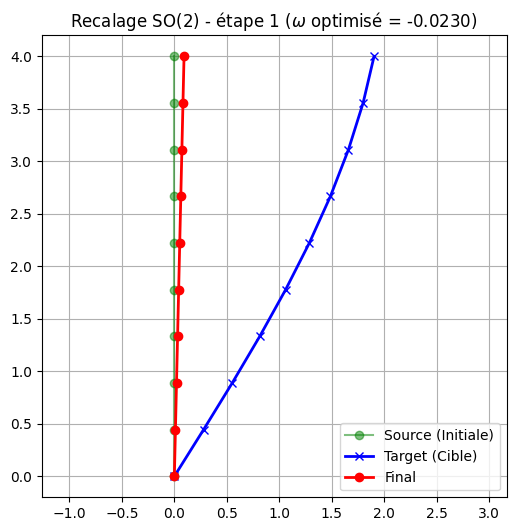
\includegraphics[width=0.48\textwidth]{../Images/RecalageRotationSO2_Etape1.png}
  \hfill
  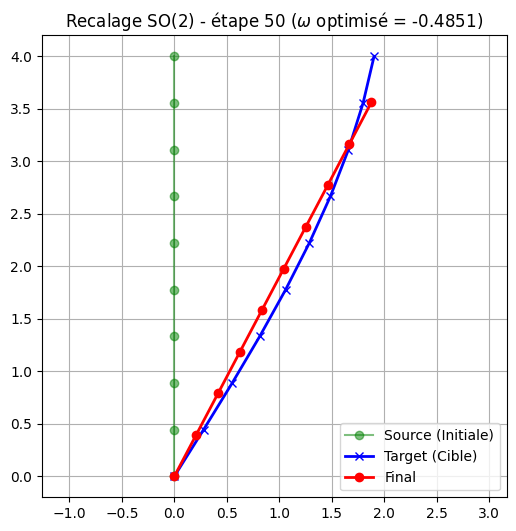
\includegraphics[width=0.48\textwidth]{../Images/RecalageRotationSO2.png}
  \caption{Première et $50^{\text{ième}}$ étape du recalage sur les rotations $SO(2)$.}\label{fig:RecalageRotationSO2}
\end{figure}
\end{exemple}

\begin{exemple}[Recalons Lecocq]\label{ex:recalage-lecocq}\leavevmode\\
Voyons des exemples de recalage par rotation sur $SO(2)$ avec des formes plus complexes.

Dans la \texttt{Figure~(\ref{fig:RecalageRotationCoq1})}, on applique une rotation à un coq $x_S$ pour le faire ``matcher'' avec la forme cible $x_T$ qui est sensiblement le même coq légèrement tourné. On voit que la figure source et cible se superposent assez bien. La géométrie du coq est préservée tout au long de la déformation, le cadre LDDMM restreint aux rotations est efficace lorsque la transformation est seulement une rotation.

\begin{figure}[H]
  \centering
  \begin{tikzpicture}
    \node[anchor=south west, inner sep=0] (main) at (0,0)
      {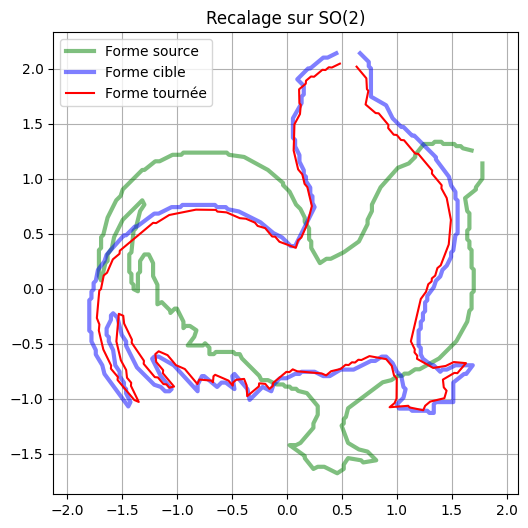
\includegraphics[width=0.42\textwidth]{../Images/RecalageRotationCoq1.png}};
    \fill[white] (0.02, 0.02) rectangle (2.4, 1.3);
    \node[anchor=south west, inner sep=0] (I0) at (0.05, 0.15)
      {\scalebox{-1}[1]{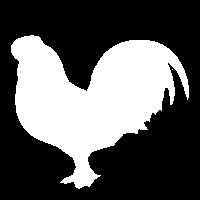
\includegraphics[width=0.06\textwidth]{../Images/coqS0.png}}};
    \node[below, font=\small] at (I0.south) {$x_S$};
    \node[anchor=south west, inner sep=0] (I1) at (1.3, 0.15)
      {\scalebox{-1}[1]{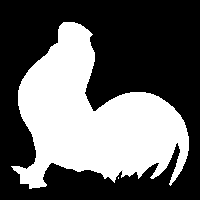
\includegraphics[width=0.06\textwidth]{../Images/coqT1.png}}};
    \node[below, font=\small] at (I1.south) {$x_T$};
    \draw[->, thick] (I0.east) -- (I1.west);
  \end{tikzpicture}
  \caption{Recalage sur les rotations $SO(2)$ d'un coq.}\label{fig:RecalageRotationCoq1}
\end{figure}

La \texttt{Figure~(\ref{fig:RecalageRotationCoq2et3})} présente deux cas où la forme cible $x_T$ diffère de la forme source $x_S$ non seulement par une rotation, mais aussi par une déformation (des coqs légèrement différents séparés de $x_S$ par une transformation non rigide). Dans ces situations, le modèle restreint à $SO(2)$ montre ses limites: en cherchant uniquement une rotation optimale, l'algorithme ne peut pas capturer les déformations non rigides. La forme transformée $x_1$ ne coïncide alors que partiellement et voire même pas du tout avec la cible $x_T$, et le terme d'attache aux données $\|x_1-x_T\|$ reste élevé malgré la convergence de l'optimisation.

\begin{figure}[H]
  \centering
  \begin{tikzpicture}
    \node[anchor=south west, inner sep=0] (main) at (0,0)
      {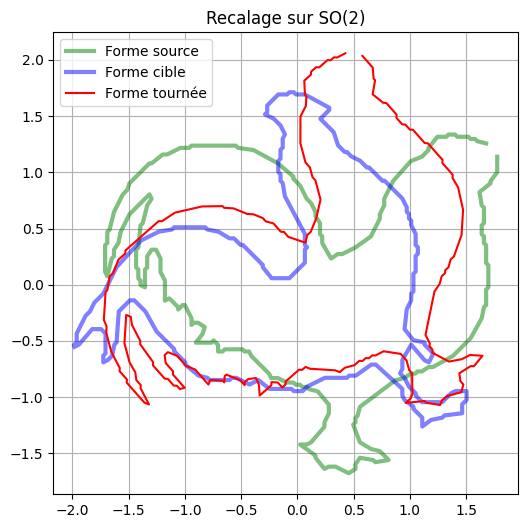
\includegraphics[width=0.42\textwidth]{../Images/RecalageRotationCoq2.png}};
    \fill[white] (0.02, 0.02) rectangle (2.4, 1.3);
    \node[anchor=south west, inner sep=0] (I0) at (0.05, 0.15)
      {\scalebox{-1}[1]{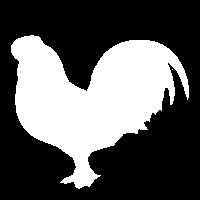
\includegraphics[width=0.06\textwidth]{../Images/coqS0.png}}};
    \node[below, font=\small] at (I0.south) {$x_S$};
    \node[anchor=south west, inner sep=0] (I1) at (1.3, 0.15)
      {\scalebox{-1}[1]{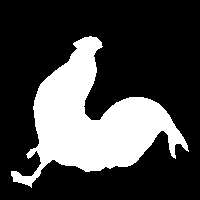
\includegraphics[width=0.06\textwidth]{../Images/coqT2.png}}};
    \node[below, font=\small] at (I1.south) {$x_T$};
    \draw[->, thick] (I0.east) -- (I1.west);
  \end{tikzpicture}
  \hfill
  \begin{tikzpicture}
    \node[anchor=south west, inner sep=0] (main) at (0,0)
      {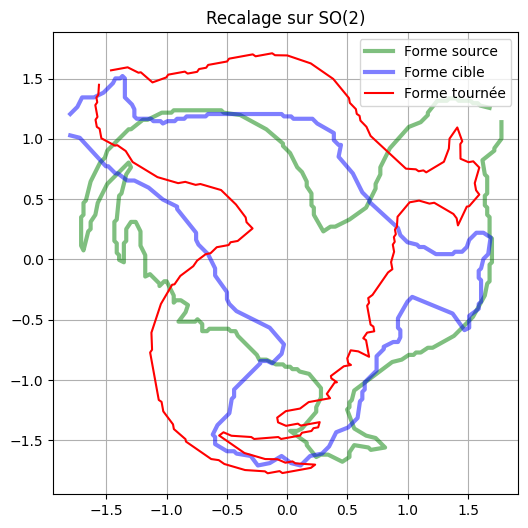
\includegraphics[width=0.42\textwidth]{../Images/RecalageRotationCoq3.png}};
    \fill[white] (0.02, 0.02) rectangle (2.4, 1.3);
    \node[anchor=south west, inner sep=0] (I0) at (0.05, 0.15)
      {\scalebox{-1}[1]{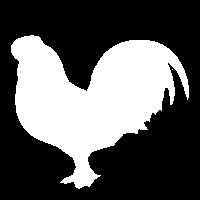
\includegraphics[width=0.06\textwidth]{../Images/coqS0.png}}};
    \node[below, font=\small] at (I0.south) {$x_S$};
    \node[anchor=south west, inner sep=0] (I1) at (1.3, 0.15)
      {\scalebox{-1}[1]{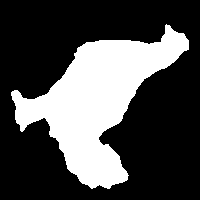
\includegraphics[width=0.06\textwidth]{../Images/coqT3.png}}};
    \node[below, font=\small] at (I1.south) {$x_T$};
    \draw[->, thick] (I0.east) -- (I1.west);
  \end{tikzpicture}
  \caption{Recalage sur les rotations $SO(2)$ de différents coqs.}\label{fig:RecalageRotationCoq2et3}
\end{figure}
\end{exemple}


\section{Approche hamiltonienne~- Tir géodésique}\label{sec:tir-hamiltonien}
On reprend maintenant la formulation hamiltonienne établie au \textbf{Chapitre~\ref{chap:Hamiltonien}} dans le cas de $N$ landmarks pour faire un algorithme de résolution par \emph{tir géodésique} (\textit{geodesic shooting})~\cite{MTT06}, où la seule variable d'optimisation est le moment initial.

\begin{proposition}[Équations géodésiques pour les nuages de points sous $SO(n)$]\label{prop:geodesique-points-reperes}\leavevmode\\
Les trajectoires optimales $(q_t,p_t)\in T^*Q$ du problème de recalage restreint à $SO(n)$ vues précédemment dans le \texttt{Chapitre~\ref{chap:Hamiltonien}} sont solutions de
\[
\begin{aligned}
\dot q_t&=A^*_t\,q_t\\
\dot p_t&=A^*_t\,p_t
\end{aligned}
\]
avec
\[
A^*_t=\frac12\left(p_t q_t^{\top}-q_t p_t^{\top}\right)\in\mathfrak{so}(n).
\]
\end{proposition}

\begin{proof}
L'équation sur $q$ s'obtient directement en substituant le contrôle optimal $A^*$ dans la dynamique $\dot q_t=A_t{q}_t$.\\
Pour l'équation sur $p$, on dérive le Hamiltonien réduit $H_r(q,p)=H(q,p,A^*(q,p))$ par rapport à $q$. Comme $A^*$ vérifie la condition d'optimalité $\partial_{A}H(q,p,A^*)=0$, la dérivée de $A^*$ par rapport à $q$ s'annule et il reste donc seulement $H$ exprimé en fonction de $q$:
\[
\partial_{q}H_r(q,p)=\partial_{q}H(q,p,A^*)={(A^*)}^{\top}p,
\]
puisque $H(q,p,A)=p^{\top}(Aq)-\frac{1}{2}\|A\|^2$ est linéaire en $q$. Les équations hamiltoniennes donnent alors
\[
\dot p_t=-\partial_{q}H_r(q_t,p_t)=-{(A^*_t)}^{\top}p_t=A^*_t\,p_t,
\]
où l'on a utilisé l'antisymétrie de $A^*_t\in\mathfrak{so}(n)$.
\end{proof}

Comme on disait juste au-dessus et donc contrairement à l'approche directe, on n'optimise plus le contrôle $\omega_t$ (ou $A_t$) le long de la trajectoire, mais uniquement la condition initiale $p_0\in{(\mathbb{R}^n)}^N$ du moment. L'algorithme est le suivant:
\begin{itemize}
  \item \textbf{Initialisation}: On choisit un moment initial:
    \[
    p_0^{(0)}=0.
    \]
  \item \textbf{Boucle d'optimisation} (pour chaque itération $k$):
  \begin{enumerate}
    \item \textit{Tir géodésique} (intégration d'Euler explicite des équations de la \textit{Proposition~\ref{prop:geodesique-points-reperes}}): En partant de $x_0=x_S$ et $p_0=p_0^{(k)}$, on intègre simultanément les deux dynamiques:
    \[
    x_{t+\Delta t}=x_t+\Delta t\,A^*_t\,x_t,\qquad p_{t+\Delta t}=p_t+\Delta t\,A^*_t\,p_t,
    \]
    où le champ optimal $A^*_t$ est recalculé à chaque pas à partir de $(x_t,p_t)$ courants. On obtient ainsi $x_1=x_1(p_0^{(k)})$ la déformation finale.
    \item \textit{Évaluation de l'énergie}: On calcule le coût global
    \[
    J(p_0^{(k)}).
    \]
    \item \textit{Mise à jour} (descente de gradient sur $p_0$): On calcule
    \[
    p_0^{(k+1)}=p_0^{(k)}-\alpha\,\nabla J(p_0^{(k)}).
    \]
  \end{enumerate}
\end{itemize}

\begin{remark}
La taille de la variable d'optimisation $p_0$ est fixée par la dimension de l'espace des formes ($nN$), indépendamment du nombre de pas de temps utilisés pour l'intégration. C'est précisément l'intérêt qu'on a mentionné au \textbf{Chapitre~\ref{chap:Hamiltonien}}: le problème de contrôle optimal, initialement posé sur un espace de contrôles $v_t$ de dimension infinie, se ramène à l'optimisation d'un unique moment initial $p_0$.
\end{remark}

\subsection{Recalage rigide sur \texorpdfstring{$SO(2)$}{SO (2)}}

\textbf{Étape 1:}\textit{ Calcul du générateur optimal}\\
La fonction \texttt{hamiltonian\_A~(\ref{code:hamiltonianA})} calcule $A^*_t=\frac12\left(p_t q_t^{\top}-q_t p_t^{\top}\right)$ à partir des tenseurs $p_t$ et $x_t$.\\

\textbf{Étape 2:}\textit{ Tir géodésique}\\
La fonction \texttt{Euler\_Hamilton~(\ref{code:EulerHamilton})} intègre simultanément $x_t$ et $p_t$ par la méthode d'Euler explicite sur $t\in[0,1]$, en réévaluant $A^*_t$ à chaque pas.\\

\textbf{Étape 3:}\textit{ Évaluation de l'énergie}\\
La fonction \texttt{hamiltonian\_loss~(\ref{code:hamiltonianloss})} calcule l'énergie totale 
\[
J(p_0)=\frac{1}{2}\|p_0\|^2+\|x_1(p_0)-x_T\|.
\]

\textbf{Étape 4:}\textit{ Mise à jour (descente de gradient sur $p_0$)}\\
La fonction \texttt{opti\_hamiltonien~(\ref{code:optihamiltonian})} optimise le moment initial $p_0$ par descente de gradient.\\

On n'illustrera pas cette partie par des exemples imagés car le changement de méthode n'impacte pas le résultat. Mais voici un exemple comparatif sur le temps d'exécution des deux méthodes.

\begin{exemple}
On compare le temps d'exécution des deux méthodes d'optimisation pour la rotation présentée en \texttt{Figure~(\ref{fig:RecalageRotationSO2})} (100 itérations de L-BFGS, mêmes points source et cible, même intégrateur d'Euler à $20$ pas de temps):
\[
t_{\text{Hamiltonien}} \approx 0.91\,\text{s}, \qquad t_{\text{Scalaire}} \approx 0.56\,\text{s}.
\]
\begin{figure}[H]
  \centering
  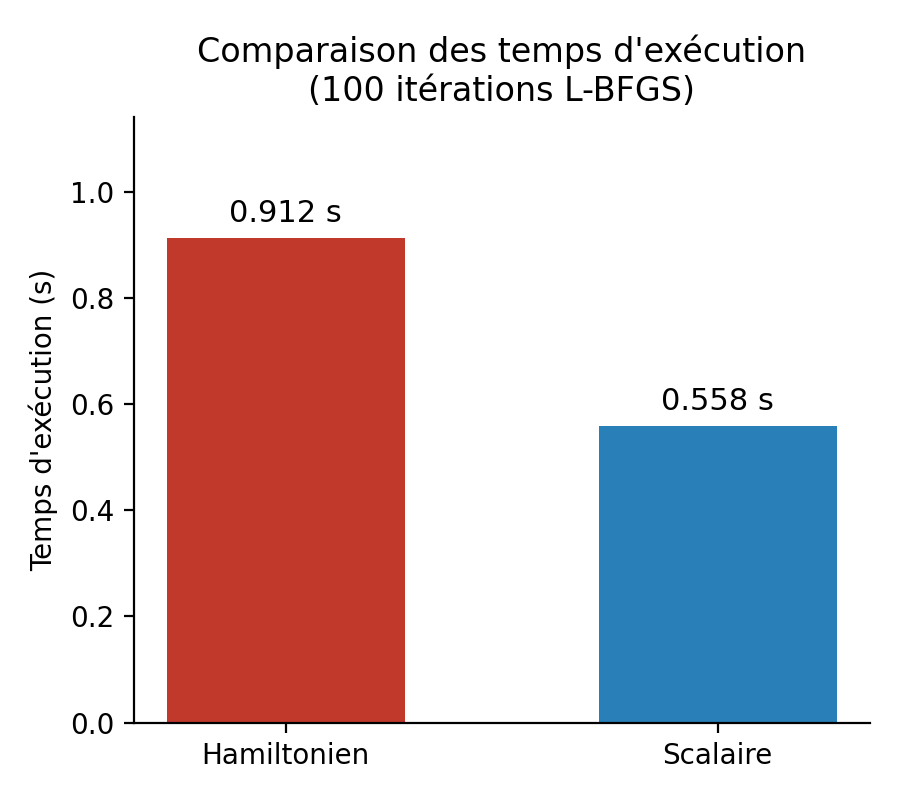
\includegraphics[width=0.48\textwidth]{../Images/DirectVsHamiltonian.png}
  \caption{Comparaison des temps d'exécution sur la rotation de la \texttt{Figure~\ref{fig:RecalageRotationSO2}}}
\end{figure}
L'approche scalaire est ici environ $1{,}6$ fois plus rapide que l'approche hamiltonienne. Cet écart s'explique par le nombre de variables intégrées à chaque pas de temps: l'approche directe ne propage que la position $x_t$, tandis que l'approche hamiltonienne propage simultanément la position $x_t$ \emph{et} le moment $p_t$, ce qui double la quantité de calcul à chaque itération d'Euler tout en recalculant $A^*_t$ à partir des deux tenseurs courants. En contrepartie, rappelons que l'approche hamiltonienne optimise un vecteur $p_0$ de même dimension que les nuages de points, ce qui la rend directement généralisable à des dynamiques bien plus riches (comme $SO(3)$ ou le cadre LDDMM général avec les difféomorphismes en dimension infinie), là où l'approche scalaire directe repose spécifiquement sur la paramétrisation par un angle $\omega$ propre à $SO(2)$.
\end{exemple}


% -= CONCLUSION =-
\chapter*{Conclusion}
\addcontentsline{toc}{chapter}{Conclusion}

Ce stage a permis d'étudier un cas particulier du recalage de formes dans lequel les transformations sont restreintes aux rotations. Après avoir rappelé le cadre général LDDMM, nous avons décrit le groupe de Lie $SO(n)$, son algèbre de Lie $\mathfrak{so}(n)$ et le rôle de l'application exponentielle pour les rotations.

La formulation hamiltonienne a constitué l'une des notions les plus challengeantes de ce travail. Le fait de comprendre que la recherche d'un champ de vitesse pouvait se ramener à l'intégration d'équations géodésiques dont la seule inconnue est le moment initial a permis d'appréhender concrètement l'intérêt du principe du maximum de Pontryagin. Les études des cas $SO(2)$ et $SO(3)$ ont rendu ces concepts plus clairs, notamment à travers les formulations simples du problème de minimisation en fonction d'un unique scalaire ou vecteur.

D'un point de vue algorithmique: les deux implémentations, l'approche directe et le tir géodésique, ont confirmé l'efficacité du modèle lorsque la transformation est une rotation rigide, en mettant aussi en évidence ses limites quand on se restreint à ces transformations ``simples''. Dès qu'interviennent des déformations non rigides, la restriction à $SO(n)$ ne permet plus de représenter correctement les transformations. Ce travail met ainsi en lumière un compromis entre la rapidité de l'approche directe et la généralité de l'approche hamiltonienne.

Plusieurs prolongements naturels sont possibles, notamment l'abandon de la limitation aux rotations afin de se rapprocher du modèle LDDMM complet, ou encore l'extension aux formes plus riches que les simples landmarks. Au-delà de ces perspectives, ce stage a surtout constitué une occasion de mettre en pratique les outils d'algèbre et d'équa-diff, vu en cours théorique, dans un contexte appliqué. Il a aussi ouvert des portes sur des domaines des mathématiques pas étudiées en $2^{\text{ème}}$ année de licence.


% -= BIBLIOGRAPHIE =-
\newpage
\bibliographystyle{plain}
\bibliography{bibliographie}
\addcontentsline{toc}{chapter}{Références}


% -= Annexe Code =-
\appendix
\chapter{Code Python}

Tout le code sera disponible sur \href{https://github.com/DJ4nto/Etude_du_groupe_de_Lie_SO_dans_le_cadre_de_l-analyse_de_formes}{ce dépôt} GitHub.

\begin{lstlisting}[caption=Fonction Euler, label=code:Euler]
def Euler(q0, omega, nt):
    dt = 1.0 / (nt - 1)
    q = q0.clone()
    A = skew_matrix(omega)
    
    Q = torch.zeros((q0.shape[0], q0.shape[1], nt), dtype=q0.dtype, device=q0.device)
    Q[:, :, 0] = q
    
    for t in range(1, nt):
        q = q + dt * (q @ A.T)
        Q[:, :, t] = q
        
    return q, Q
\end{lstlisting}

\begin{lstlisting}[caption=Fonction rotation\_loss, label=code:rotation_loss]
def rotation_loss(dataloss_fnc, nt):
    def loss(q0, omega):
        q_final, _ = Euler(q0, omega, nt)
        dloss = dataloss_fnc(q_final)
        reg = 0.5 * (omega ** 2)
        return reg + dloss
    return loss
\end{lstlisting}

\begin{lstlisting}[caption=Fonction opti\_rotation, label=code:opti_rotation]
def opti_rotation(q0, loss_fnc, n_iter, eta):
    omega = torch.zeros(1, dtype=q0.dtype, device=q0.device, requires_grad=True)
    optimizer = torch.optim.LBFGS([omega], lr=eta, line_search_fn='strong_wolfe')
    losses = []

    def closure():
        optimizer.zero_grad()
        L = loss_fnc(q0, omega)
        L.backward()
        return L

    for i in range(n_iter):
        L = optimizer.step(closure)
        losses.append(L.item())

    return omega.detach(), losses
\end{lstlisting}

\begin{lstlisting}[caption=Fonction hamiltonian\_A, label=code:hamiltonianA]
def hamiltonian_A(p, q):
    return 0.5 * (p.T @ q - q.T @ p)
\end{lstlisting}

\begin{lstlisting}[caption=Fonction Euler\_Hamilton, label=code:EulerHamilton]
def Euler_Hamilton(q0, p0, nt):
    dt = 1.0 / (nt - 1)
    q = q0.clone()
    p = p0.clone()
    Q = torch.zeros((q0.shape[0], q0.shape[1], nt), dtype=q0.dtype, device=q0.device)
    P = torch.zeros((p0.shape[0], p0.shape[1], nt), dtype=p0.dtype, device=p0.device)
    Q[:, :, 0] = q
    P[:, :, 0] = p

    for t in range(1, nt):
        A = hamiltonian_A(p, q)
        q = q + dt * (q @ A.T)
        p = p + dt * (p @ A.T)
        Q[:, :, t] = q
        P[:, :, t] = p

    return q, p, Q, P
\end{lstlisting}

\begin{lstlisting}[caption=Fonction hamiltonian\_loss, label=code:hamiltonianloss]
def hamiltonian_loss(dataloss_fnc, nt):
    def loss(q0, p0):
        q_final, p_final, _, _ = Euler_Hamilton(q0, p0, nt)
        dloss = dataloss_fnc(q_final)
        reg = 0.5 * (p0 ** 2).sum()
        return reg + dloss
    return loss
\end{lstlisting}

\begin{lstlisting}[caption=Fonction opti\_hamiltonian, label=code:optihamiltonian]
def opti_hamiltonian(q0, loss_fnc, n_iter, eta):
    p0 = torch.zeros_like(q0, requires_grad=True)
    optimizer = torch.optim.LBFGS([p0], lr=eta, line_search_fn='strong_wolfe')
    losses = []

    def closure():
        optimizer.zero_grad()
        L = loss_fnc(q0, p0)
        L.backward()
        return L

    for i in range(n_iter):
        L = optimizer.step(closure)
        losses.append(L.item())

        print(f"Iteration {i+1:3d} - Loss: {L.item():.6f} | |p0|: {p0.norm().item():.4f}")
        print(f"")

    return p0.detach(), losses
\end{lstlisting}


% -= Annexe Images =-
\chapter{Figures supplémentaires}

Quelques figures supplémentaires.

\begin{figure}[H]
  \centering
  \begin{tikzpicture}
    \node[anchor=south west, inner sep=0] (main) at (0,0)
      {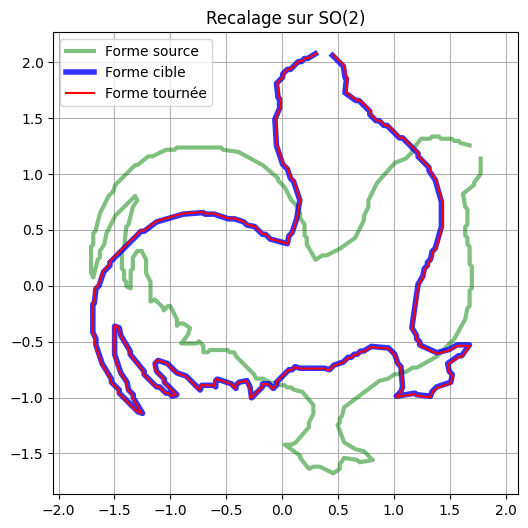
\includegraphics[width=0.42\textwidth]{../Images/RecalageRotationCoq0.png}};
    \fill[white] (0.02, 0.02) rectangle (2.4, 1.3);
    \node[anchor=south west, inner sep=0] (I0) at (0.05, 0.15)
      {\scalebox{-1}[1]{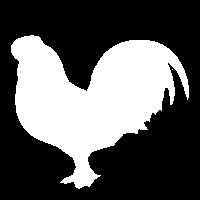
\includegraphics[width=0.06\textwidth]{../Images/coqS0.png}}};
    \node[below, font=\small] at (I0.south) {$x_S$};
    \node[anchor=south west, inner sep=0] (I1) at (1.3, 0.15)
      {\scalebox{-1}[1]{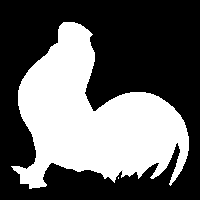
\includegraphics[width=0.06\textwidth]{../Images/coqT1.png}}};
    \node[below, font=\small] at (I1.south) {$x_T$};
    \draw[->, thick] (I0.east) -- (I1.west);
  \end{tikzpicture}
  \caption{Complète l'exemple~(\ref{ex:recalage-rigide-coq})}
\end{figure}
\begin{figure}[H]
  \centering
  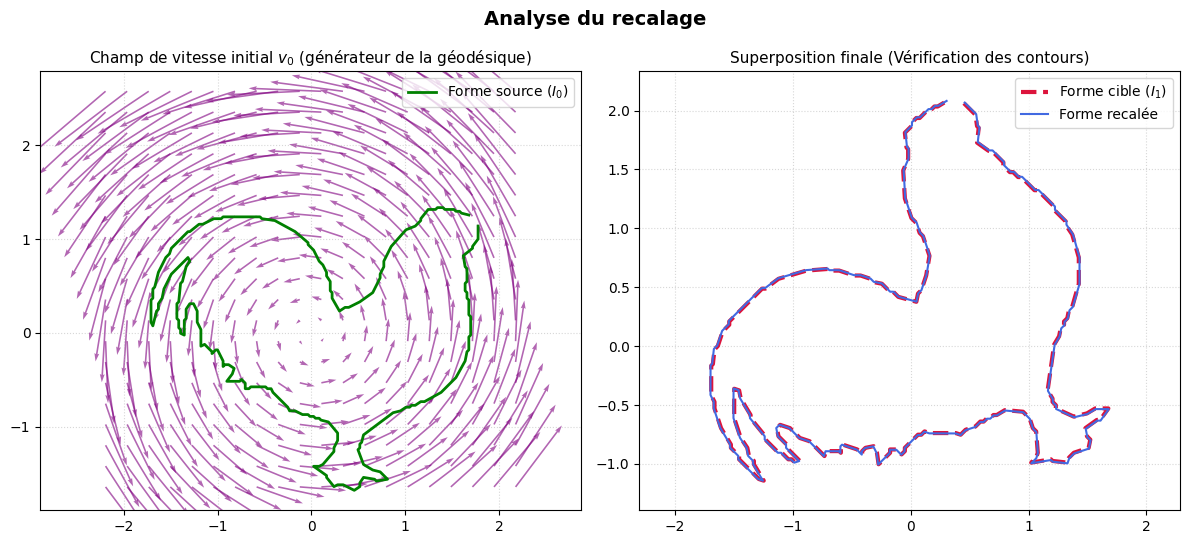
\includegraphics[width=1\textwidth]{../Images/AnalyseRecalageCoq0.png}
  \caption{Complète l'exemple~(\ref{ex:recalage-rigide-coq})}
\end{figure}

\begin{figure}[H]
  \centering
  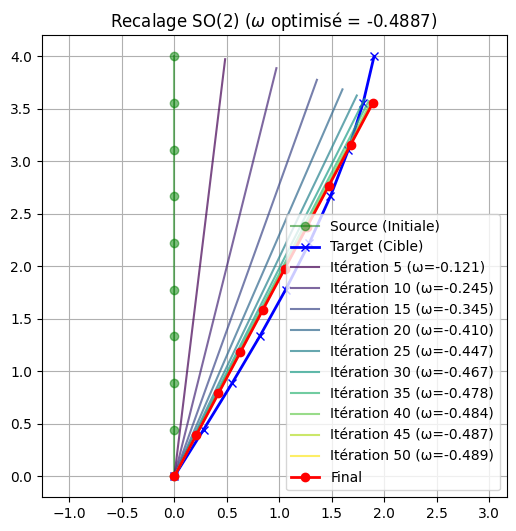
\includegraphics[width=1\textwidth]{../Images/EvolutionRecalageRotationSO2.png}
  \caption{Complète l'exemple~(\ref{ex:recalage-barre})}
\end{figure}

\begin{figure}[H]
  \centering
  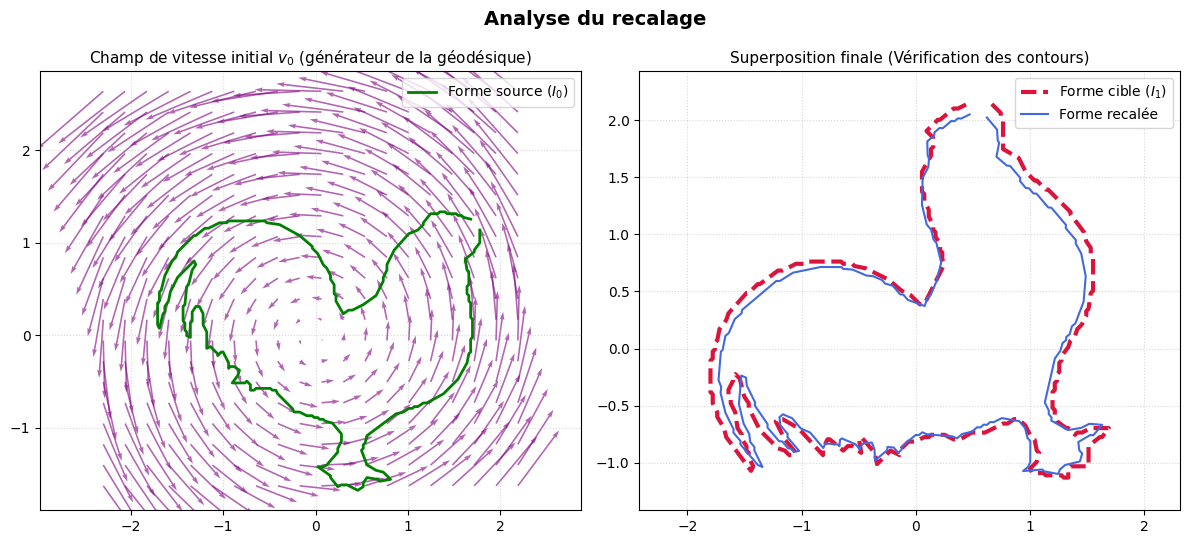
\includegraphics[width=1\textwidth]{../Images/AnalyseRecalageCoq1.png}
  \caption{Complète l'exemple~(\ref{ex:recalage-lecocq})}
\end{figure}
\begin{figure}[H]
  \centering
  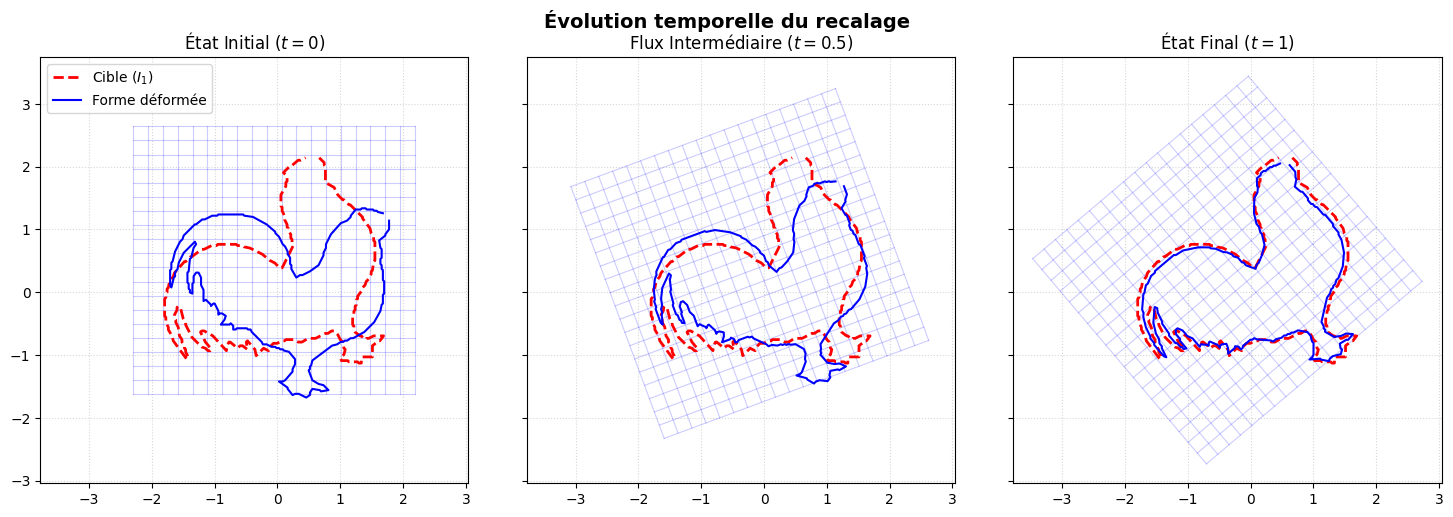
\includegraphics[width=1\textwidth]{../Images/EvolutionRecalageCoq1.png}
  \caption{Complète l'exemple~(\ref{ex:recalage-lecocq})}
\end{figure}
\begin{figure}[H]
  \centering
  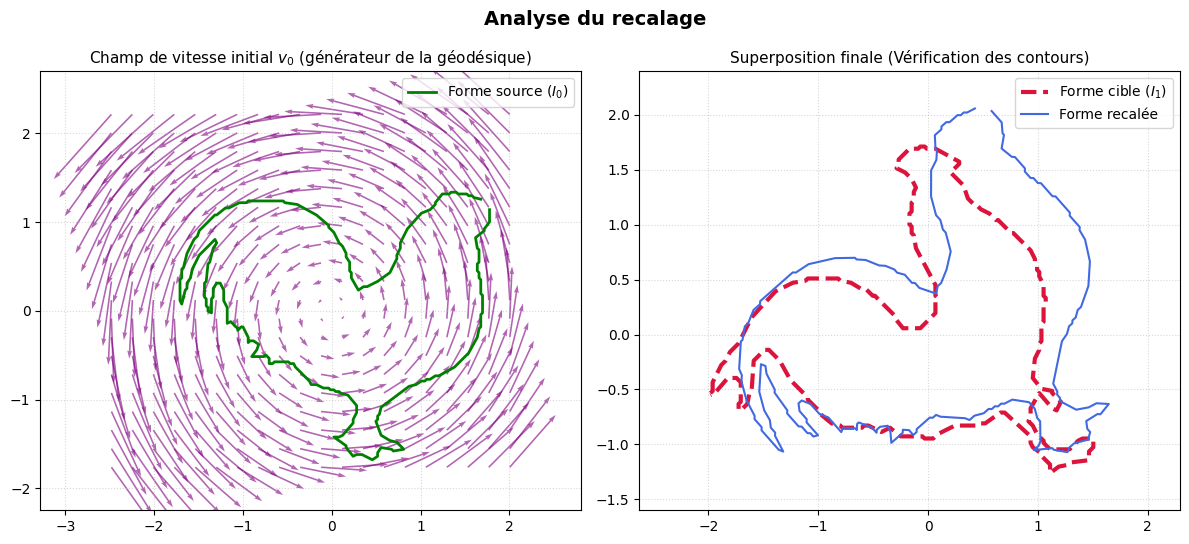
\includegraphics[width=1\textwidth]{../Images/AnalyseRecalageCoq2.png}
  \caption{Complète l'exemple~(\ref{ex:recalage-lecocq})}
\end{figure}
\begin{figure}[H]
  \centering
  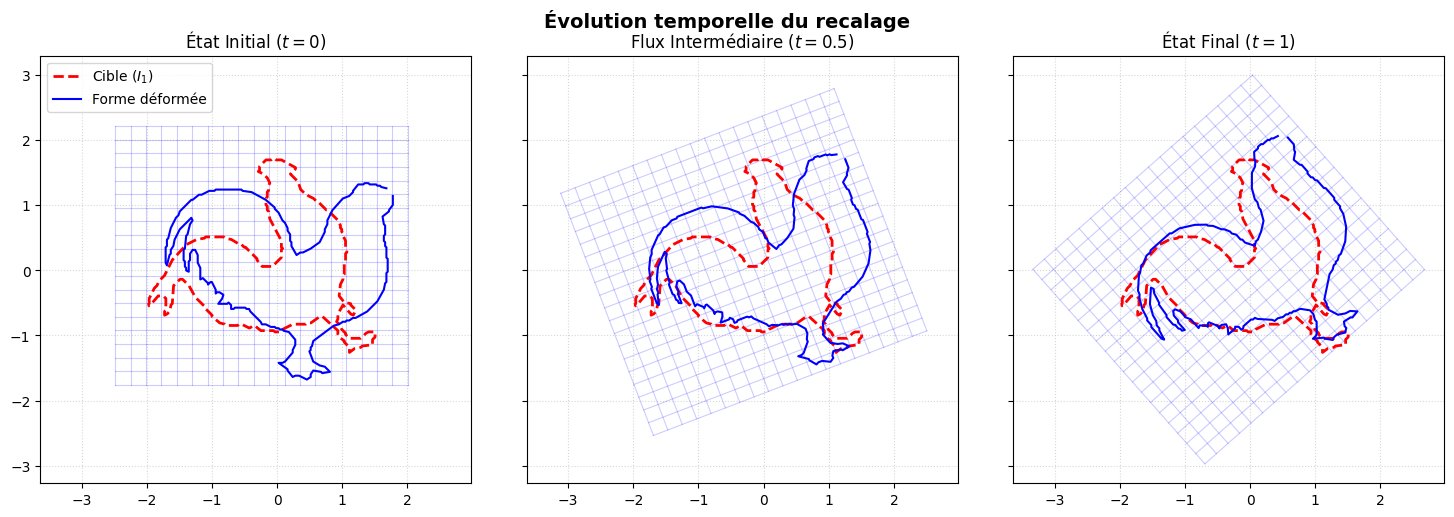
\includegraphics[width=1\textwidth]{../Images/EvolutionRecalageCoq2.png}
  \caption{Complète l'exemple~(\ref{ex:recalage-lecocq})}
\end{figure}
\begin{figure}[H]
  \centering
  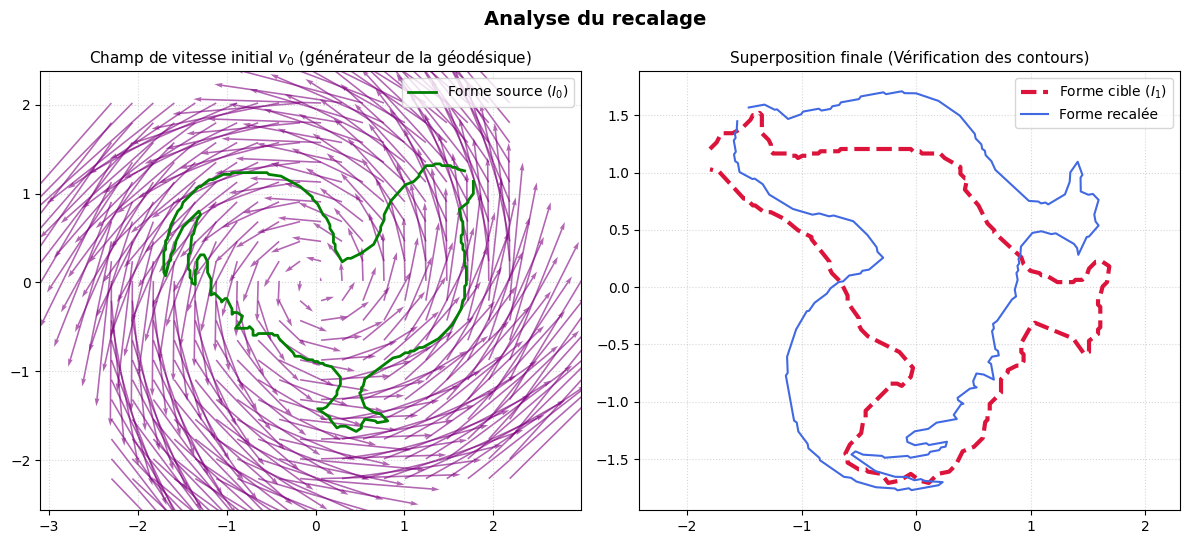
\includegraphics[width=1\textwidth]{../Images/AnalyseRecalageCoq3.png}
  \caption{Complète l'exemple~(\ref{ex:recalage-lecocq})}
\end{figure}
\begin{figure}[H]
  \centering
  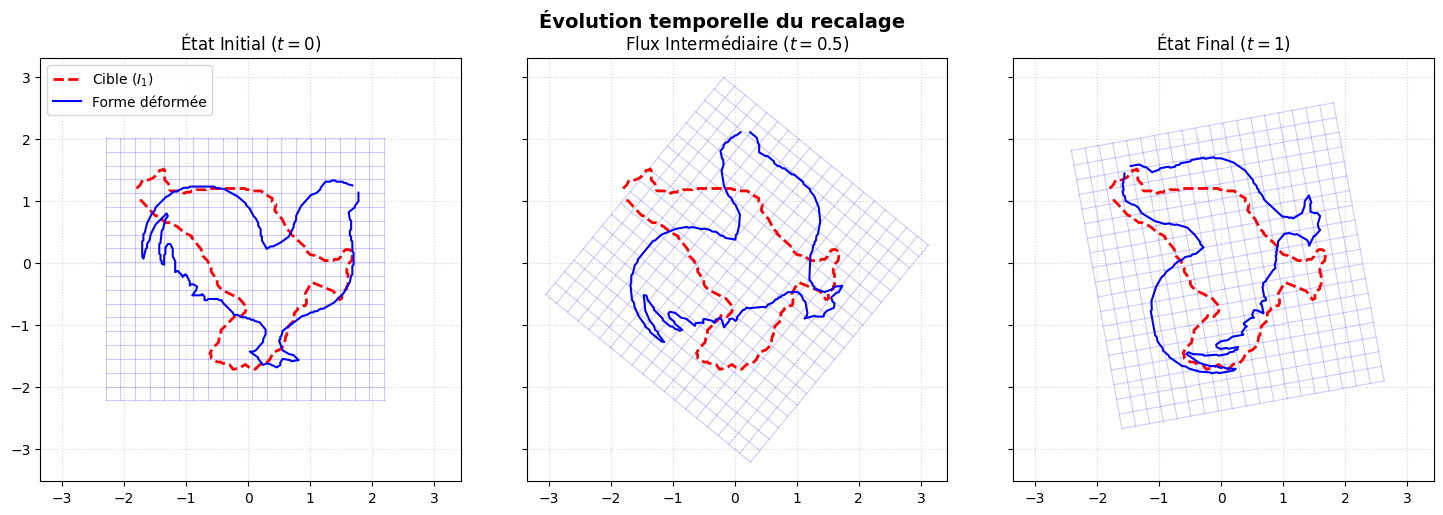
\includegraphics[width=1\textwidth]{../Images/EvolutionRecalageCoq3.png}
  \caption{Complète l'exemple~(\ref{ex:recalage-lecocq})}
\end{figure}

\end{document}
